\باب{بلند درجی خطی سادہ تفرقی مساوات}
دو درجی خطی سادہ تفرقی مساوات کو حل کرنے کے طریقے بلند درجی خطی سادہ تفرقی مساوات کے لئے بھی قابل استعمال ہیں۔ہم دیکھیں گے کہ بلند درجی صورت میں مساوات زیادہ پیچیدہ ہوں گے،  امتیازی مساوات کے جذر بھی تعداد میں زیادہ اور حصول میں نسبتاً مشکل ہوں گے اور ورونسکی زیادہ اہم کردار ادا کرے گا۔ 

\حصہ{متجانس خطی سادہ تفرقی مساوات}
\عددی{n} درجی سادہ تفرقی مساوات سے مراد ایسی مساوات ہے جس میں نا معلوم متغیرہ \عددی{y(x)} کا \عددی{y^n=\tfrac{\dif^{\, n} y}{\dif x^n}} سب سے بلند درجی تفرق ہو۔ایسی سادہ تفرقی مساوات کو
\begin{align*}
F(x,y,y',\cdots, y^{(n)})=0
\end{align*}
لکھا جا سکتا ہے جس میں \عددی{y} اور کم درجی تفرق موجود یا غیر موجود ہو سکتے ہیں۔ایسی مساوات کو \اصطلاح{خطی}\فرہنگ{خطی}\فرہنگ{linear} کہتے ہیں اگر اس کو 
\begin{align}\label{مساوات_سادہ_بلند_خطی_الف}
y^{(n)}+p_{n-1}(x)y^{(n-1)}+\cdots+p_1(x)y'+p_0(x)y=r(x)
\end{align}
لکھنا ممکن ہو۔صفحہ \حوالہصفحہ{مساوات_سادہ_دو_درجی_تعریف} پر دو درجی خطی سادہ تفرقی مساوات کی بات کی گئی۔موجودہ مساوات میں \عددی{n=2}، \عددی{p_1=p} اور \عددی{p_0=q} پر کرنے سے دو درجی مساوات حاصل ہو گی۔عددی سر \عددی{p_0(x)} تا \عددی{p_n(x)}  اور جبری تفاعل \عددی{r(x)} غیر تابع متغیرہ  \عددی{x} کے کوئی بھی تفاعل ہو سکتے ہیں جبکہ \عددی{y(x)} نا معلوم متغیرہ ہے۔خطی مساوات کو معیاری صورت میں لکھا گیا ہے جہاں \عددی{y^{(n)}} کا عددی سر اکائی \عددی{1} ہے۔ تفرقی مساوات میں  \عددی{p_n(x)y^{(n)}} موجود ہونے کی صورت میں پوری مساوات کو \عددی{p_n(x)} سے تقسیم کرتے ہوئے معیاری صورت حاصل کریں۔جو تفرقی مساوات درج بالا صورت میں لکھنا ممکن نہ ہو \اصطلاح{غیر خطی}\فرہنگ{غیر خطی}\فرہنگ{non linear} کہلاتی ہے۔

کسی کھلے وقفے \عددی{I} پر \عددی{r(x)} \اصطلاح{مکمل صفر}\فرہنگ{مکمل صفر} \عددی{r \equiv 0} ہونے کی صورت میں  مساوات \حوالہ{مساوات_سادہ_بلند_خطی_الف} سے \اصطلاح{متجانس مساوات}\فرہنگ{متجانس مساوات}\فرہنگ{homogeneous}
\begin{align}\label{مساوات_سادہ_بلند_خطی_ب}
y^{(n)}+p_{n-1}(x)y^{(n-1)}+\cdots+p_1(x)y'+p_0(x)y=0
\end{align}
حاصل ہوتی ہے۔کھلے وقفے پر \عددی{r(x)} کے مکمل صفر ہونے سے مراد یہ ہے کہ اس وقفے پر ہر \عددی{x} کے لئے \عددی{r(x)} کی قیمت صفر کے برابر ہے۔دو درجی تفرقی مساوات کی طرح  اگر \عددی{r(x)} مکمل صفر نہ ہو تب مساوات \اصطلاح{غیر متجانس}\فرہنگ{غیر متجانس}\فرہنگ{nonhomogeneous} کہلائے گی۔

کھلے وقفہ \عددی{I} پر \عددی{n} درجی خطی یا غیر خطی سادہ تفرقی مساوات کے حل \عددی{y=h(x)} سے مراد ایسا تفاعل ہے جو \عددی{I} پر معین ہو،  کھلے وقفے پر اس کا \عددی{n} درجی تفرق موجود ہو اور تفرقی مساوات میں \عددی{y} اور اس کے تفرقات کی جگہ \عددی{h} اور اس کے تفرقات پر کرنے سے مساوات کے دونوں اطراف بالکل یکساں حاصل ہوں۔ 
%=======================

\جزوحصہء{متجانس خطی سادہ تفرقی مساوات:خطی میل اور عمومی حل}
\اصطلاح{خطی میل}\فرہنگ{خطی میل} یا \اصطلاح{اصول خطیت}\فرہنگ{اصول خطیت} جس کا ذکر صفحہ \حوالہصفحہ{مسئلہ_دو_درجی_خطی_میل} مسئلہ \حوالہ{مسئلہ_دو_درجی_خطی_میل} میں کیا گیا بلند درجی خطی متجانس سادہ تفرقی مساوات کے لئے بھی درست ہے۔
%===============

\ابتدا{مسئلہ}\quad بنیادی مسئلہ برائے متجانس خطی سادہ بلند درجی تفرقی مساوات\فرہنگ{مسئلہ!بنیادی۔متجانس خطی}\\
کھلے وقفہ \عددیء{I} پر متجانس خطی بلند درجی تفرقی مساوات \حوالہ{مساوات_سادہ_بلند_خطی_ب} کے حل کا خطی میل بھی \عددیء{I} پر اس مساوات کا حل ہو گا۔بالخصوص ان حل کو مستقل مقدار سے ضرب دینے سے بھی مساوات کے حل حاصل ہوتے ہیں۔(یہ اصول غیر خطی اور  غیر متجانس مساوات پر لاگو نہیں ہوتا۔)
\انتہا{مسئلہ}
%==========================

اس کا ثبوت گزشتہ باب میں دئے گئے ثبوت کی طرح ہے جس کو یہاں پیش نہیں کیا جائے گا۔

ہماری بقایا گفتگو ہو بہو دو درجی تفرقی مساوات کی طرح ہو گی لہٰذا یہاں بلند درجی خطی متجانس مساوات کی عمومی حل کی بات کرتے ہیں۔ایسا کرنے کی خاطر \عددی{n} عدد تفاعل کی  \اصطلاح{خطی طور غیر تابع}\فرہنگ{غیر تابع!خطی طور}\فرہنگ{خطی طور!غیر تابع} ہونے کی تصور کو وسعت دیتے ہیں۔

%====================
\ابتدا{تعریف}\quad عمومی حل، اساس اور مخصوص حل\\
کھلے وقفے \عددی{I} پر مساوات \حوالہ{مساوات_سادہ_بلند_خطی_ب} کا \اصطلاح{عمومی حل}\فرہنگ{عمومی حل}\فرہنگ{general solution}
\begin{align}
y(x)=c_1y_1(x)+c_2y_2(x)+\cdots +c_ny_n(x)
\end{align}
ہے جہاں \عددی{y_1(x)} تا \عددی{y_n(x)} حل کی اساس اور \عددی{c_1} تا \عددی{c_2} اختیاری مستقل ہیں۔یوں \عددی{y_1} تا \عددی{y_n} کھلے وقفے پر خطی طور غیر تابع ہیں۔ 

عمومی حل کے مستقل کی قیمتیں مقرر کرنے سے \اصطلاح{مخصوص حل}\فرہنگ{مخصوص حل}\فرہنگ{particular solution} حاصل ہو گا۔
\انتہا{تعریف}
%=========================

\ابتدا{تعریف}\quad خطی طور تابع تفاعل اور خطی طور غیر تابع تفاعل\\
تصور کریں کہ کھلے وقفے \عددی{I} پر  \عددی{n} عدد تفاعل \عددی{y_1(x)} تا \عددی{y_n(x)} معین ہیں۔

 وقفہ \عددی{I} پر معین \عددی{y_1} تا \عددی{y_n}،  اس وقفے   پر اس صورت \اصطلاح{خطی طور غیر تابع}\فرہنگ{خطی طور! غیر تابع}\حاشیہب{linearly independent}\فرہنگ{linearly independent} کہلاتے ہیں جب پورے وقفے پر
\begin{align}\label{مساوات_سادہ_بلند_خطی_طور_غیر_تابع_الف}
k_1 y_1(x)+k_2 y_2(x)+\cdots+k_ny_n(x)=0
\end{align}
سے مراد 
\begin{align*}
k_1=k_2= \cdots =k_n=0 
\end{align*}
ہو۔\عددی{k_1} تا \عددی{k_n} میں  کم از کم ایک کی قیمت صفر نہ ہونے کی صورت میں مساوات \حوالہ{مساوات_سادہ_بلند_خطی_طور_غیر_تابع_الف} پر پورا اترتے ہوئے حل \عددی{y_1} تا \عددی{y_n} \اصطلاح{خطی طور تابع}\فرہنگ{خطی طور!تابع}\حاشیہب{linearly dependent}\فرہنگ{linearly dependent} کہلاتے ہیں۔
\انتہا{تعریف}
%==========================

\عددی{y_1} تا \عددی{y_n} میں (کم از کم ایک) تفاعل کو اس صورت بقایا تفاعل کے \اصطلاح{خطی میل}\فرہنگ{خطی میل} کے طرز پر لکھا جا سکتا ہے جب اس وقفے پر \عددی{y_1} تا \عددی{y_n} خطی طور تابع ہوں۔ یوں اگر \عددی{k_1 \ne 0} ہو تب ہم مساوات \حوالہ{مساوات_سادہ_بلند_خطی_طور_غیر_تابع_الف} کو \عددی{k_1} سے تقسیم کرتے ہوئے
\begin{align*}
y_1=-\frac{1}{k_1}(k_2 y_2+k_3y_3+\cdots+k_ny_n)
\end{align*}
 لکھ سکتے ہیں جو تناسبی رشتہ ہے۔یہ مساوات کہتی ہے کہ \عددی{y_1} کو بقایا تفاعل کے خطی میل کی صورت میں لکھا جا سکتا ہے۔اسی کو خطی طور تابع کہتے ہیں۔آپ دیکھ سکتے ہیں کہ \عددی{n=2} کی صورت میں ہمیں حصہ \حوالہ{حصہ_سادہ_دو_وجودیت_یکتائی_ورونسکی} میں بیان کئے گئے تصورات ملتے ہیں۔
%=======================

\ابتدا{مثال}\quad خطی طور تابع\\
ثابت کریں کہ تفاعل \عددی{y_1=2\sin x}، \عددی{y_2=1.5x^2}، \عددی{y_3=5\cos x+\sin x} اور \عددی{y_4=4\cos x} کسی بھی کھلے وقفے پر خطی طور تابع ہیں۔

حل:ہم \عددی{y_3=\tfrac{1}{2}y_1+0y_2+\tfrac{5}{4}y_4} لکھ سکتے ہیں لہٰذا \عددی{y_1} تا \عددی{y_4} خطی طور تابع تفاعل ہیں۔
\انتہا{مثال}
%============================
\ابتدا{مثال}\شناخت{مثال_سادہ_بلند_خطی_طور_غیر_تابع}\quad خطی طور غیر تابع\\
ثابت کریں کہ \عددی{y_1=x}، \عددی{y_2=x^3} اور \عددی{y=x^4}  کسی بھی کھلے وقفے پر خطی طور غیر تابع ہیں۔

حل:ہم  مساوات \عددی{k_1y_1+k_2y_2+k_3y_3=0} میں مختلف \عددی{x} کی قیمتیں پر کرتے ہوئے \عددی{k_1} تا \عددی{k_3} دریافت کرتے ہیں۔کھلے وقفے پر نقطہ \عددی{x=1}، \عددی{x=-1} اور \عددی{x=2} چنتے ہوئے درج ذیل ہمزاد مساوات ملتے ہیں۔
\begin{align*}
k_1+k_2+k_3&=0\\
-k_1-k_2+k_3&=0\\
2k_1+8k_2+16k_3&=0
\end{align*}
ان ہمزاد مساوات کو حل کرتے ہوئے \عددی{k_1=0}، \عددی{k_2=0} اور \عددی{k_3=0} ملتا ہے جو خطی طور غیر تابع ہونے کا ثبوت ہے۔
\انتہا{مثال}
%========================
\ابتدا{مثال}\شناخت{مثال_سادہ_بلند_اساس_عمومی_حل_الف}\quad اساس۔عمومی حل\\
تین درجی سادہ تفرقی مساوات \عددی{y^{(3)}-y'=0} کا عمومی حل تلاش کریں۔ \عددی{y^{(3)}} سے مراد \عددی{\tfrac{\dif^{\,3} y}{\dif x^3}} ہے۔

حل:حصہ \حوالہ{حصہ_سادہ_دو_درجی_مستقل_عددی_سر} کی طرح ہم اس متجانس مساوات کا حل \عددی{y=e^{\lambda x}} تصور کرتے  ہوئے امتیازی مساوات
\begin{align*}
\lambda^3-\lambda=0
\end{align*}
حاصل کرتے ہیں۔اس کو \عددی{\lambda(\lambda^2-1)=0} لکھتے ہوئے \عددی{\lambda=0} اور \عددی{\lambda=\mp 1} ملتے ہیں جن سے اساس \عددی{y_1=c}، \عددی{y_2=e^x} اور \عددی{y_3=e^{-x}} ملتا ہے۔جیسا مثال \حوالہ{مثال_سادہ_بلند_اساس_عمومی_حل_ب} میں ثابت کیا جائے گا، یہ اساس کسی بھی کھلے وقفے پر خطی طور غیر تابع ہیں لہٰذا کسی بھی کھلے وقفے پر  عمومی حل 
\begin{align*}
y=c_1+c_2e^x+c_3e^{-x}
\end{align*}
ہو گا۔
\انتہا{مثال}
%=======================

\جزوحصہء{ابتدائی قیمت مسئلہ۔وجودیت اور یکتائی}
مساوات \حوالہ{مساوات_سادہ_بلند_خطی_ب} پر مبنی ابتدائی قیمت مسئلہ مساوات \حوالہ{مساوات_سادہ_بلند_خطی_ب} اور درج ذیل \عددی{n} \اصطلاح{ابتدائی شرائط}\فرہنگ{ابتدائی!شرائط} پر مشتمل ہو گا
\begin{align}\label{مساوات_سادہ+بلند_ابتدائی_شرائط}
y(x_0)=K_0, y'(x_0)=K_1,\cdots , y^{(n-1)}(x_0)=K_{n-1}
\end{align}
جہاں \عددی{x_0} کھلے وقفے \عددی{I} پر ایک نقطہ اور \عددی{K_0} تا \عددی{K_{n-1}} اس نقطے پر  دیے گئے مقدار ہیں۔

صفحہ \حوالہصفحہ{مسئلہ_سادہ_دو_درجی_یکتا_مخصوص_حل} پر مسئلہ \حوالہ{مسئلہ_سادہ_دو_درجی_یکتا_مخصوص_حل} کو وسعت دیتے ہیں جس سے درج ذیل ملتا ہے۔
%============================

\ابتدا{مسئلہ}\شناخت{مسئلہ_سادہ_بلند_درجی_یکتا_مخصوص_حل}\quad مسئلہ وجودیت اور یکتائی برائے ابتدائی قیمت بلند درجی  تفرقی مساوات\فرہنگ{مسئلہ!وجودیت اور یکتائی}\\
کھلے وقفہ \عددی{I} پر مساوات \حوالہ{مساوات_سادہ_بلند_خطی_ب} کے عددی سر \عددی{p_0} تا \عددی{p_{n-1}} استمراری ہونے کی صورت میں اگر \عددی{x_0} کھلے وقفے پر پایا جاتا ہو تب مساوات \حوالہ{مساوات_سادہ_بلند_خطی_ب} اور مساوات \حوالہ{مساوات_سادہ+بلند_ابتدائی_شرائط} پر مبنی ابتدائی قیمت مسئلے کا \عددی{I} پر  \اصطلاح{یکتا حل}\فرہنگ{یکتا حل} \عددی{y(x)} \اصطلاح{موجود}\فرہنگ{حل!موجود}\فرہنگ{موجود!حل} ہے۔
\انتہا{مسئلہ}
%============================

حل کی موجودگی کا ثبوت اس کتاب میں نہیں دیا جائے گا۔کتاب کے آخر میں ضمیمہ \حوالہ{ضمیمہ_اضافی_ثبوت} میں  حل کی یکتائی کے ثبوت میں معمولی رد بدل سے یکتائی ثابت کی جا سکتی ہے۔  

%================
\ابتدا{مثال}\quad تین درجی یولر کوشی مساوات کا ابتدائی قیمت مسئلہ\\
درج ذیل ابتدائی قیمت مسئلے کو حل کریں۔
\begin{align*}
x^3y'''-5x^2y''+12xy'-12y=0,\quad y(1)=1, \quad y'(1)=-1, \quad y''(1)=0
\end{align*}

حل:ہم تفرقی مساوات میں آزمائشی تفاعل \عددی{y=x^m} پر کرتے ہوئے امتیازی مساوات
\begin{align*}
m^3-8m^2+19m-12=0
\end{align*}
حاصل کرتے ہیں جس کے جذر \عددی{m=1}، \عددی{m=3} اور \عددی{m=4} ہیں۔جذر  کو مختلف طریقوں سے حاصل کیا جاتا ہے البتہ یہاں جذر حاصل کرنے پر بحث نہیں کی جائے گی۔ یوں حل کی اساس \عددی{y_1=x}، \عددی{y_2=x^3} اور \عددی{y_3=x^4} ہیں جنہیں مثال \حوالہ{مثال_سادہ_بلند_خطی_طور_غیر_تابع} میں خطی طور غیر تابع ثابت کیا گیا۔اس طرح عمومی حل
\begin{align*}
y=c_1x+c_2x^3+c_3x^4
\end{align*}
ہو گا۔دیے گئے تفرقی مساوات کو  \عددی{x^3} سے تقسیم کرتے ہوئے \عددی{y'''} کا عددی سر اکائی حاصل کرتے ہوئے تفرقی مساوات کی معیاری صورت حاصل ہوتی ہے۔معیاری صورت میں مساوات کے دیگر عددی سر \عددی{x=0} پر غیر استمراری ہیں۔اس کے باوجود درج بالا عمومی حل تمام \عددی{x} بشمول  \عددی{x=0} کے لئے درست ہے۔ 

عمومی حل اور اس کے تفرقات \عددی{y'=c_1+3c_2x^2+4c_3x^3} اور \عددی{y''=6c_2x+12c_3x^2} میں ابتدائی معلومات پر کرتے ہوئے درج ذیل ہمزاد مساوات ملتے ہیں
\begin{align*}
c_1+c_2+c_3&=1\\
c_1+3c_2+4c_3&=-1\\
6c_2+12c_3&=0
\end{align*}
جن کا حل \عددی{c_1=3}، \عددی{c_2=-4} اور \عددی{c_3=2} ہے۔اس طرح مخصوص حل درج ذیل ہو گا۔
\begin{align*}
y=3x-4x^3+2x^4
\end{align*}
\انتہا{مثال}
%==========================

\جزوحصہء{خطی طور غیر تابع حل۔ورونسکی}
عمومی حل کے حصول کے لئے ضروری ہے کہ حل خطی طور غیر تابع ہوں۔اگرچہ عموماً حل کو دیکھ کر ہی اندازہ ہو جاتا ہے کہ  وہ خطی طور غیر تابع ہیں یا نہیں ہیں، البتہ ایسا معلوم کرنے کا منظم طریقہ زیادہ بہتر ہو گا۔صفحہ \حوالہصفحہ{مسئلہ_سادہ_دو_حل_تابع_غیر_تابع} پر مسئلہ \حوالہ{مسئلہ_سادہ_دو_حل_تابع_غیر_تابع} دو درجی  \عددی{n=2} مساوات کے علاوہ بلند درجی مساوت کے لئے بھی درست ہے۔ بلند درجی مساوات کی صورت میں ورونسکی درج ذیل ہو گی۔
\begin{align}\label{مساوات_سادہ_بلند_ورونسکی_الف}
W(y_1,\cdots, y_n)=
\begin{vmatrix}
y_1 & y_2 & \cdots & y_n\\
y'_1 & y'_2 & \cdots & y'_n\\
\vdots & & \\
y_1^{(n-1)} & y_2^{(n-1)} & \cdots & y_n^{(n-1)}
\end{vmatrix}
\end{align}
ورونسکی تفرقی مساوات کے حل \عددی{y_1} تا \عددی{y_n} پر مبنی ہے جو از خود \عددی{x} پر مبنی ہیں۔ورونسکی غیر صفر ہونے کی صورت میں  \عددی{y_1} تا \عددی{y_n} خطی طور غیر تابع ہوں گے۔
%========================

\ابتدا{مسئلہ}\شناخت{مسئلہ_سادہ_بلند_حل_تابع_غیر_تابع}\quad خطی طور تابع اور غیر تابع حل\فرہنگ{مسئلہ!تابع اور غیر تابع حل}\\
کھلے وقفہ \عددی{I} پر استمراری  \عددی{p_0(x)} تا  \عددی{p_{n-1}(x)} عددی سر والے سادہ تفرقی  مساوات \حوالہ{مساوات_سادہ_بلند_خطی_ب} کے \عددی{I}  پر حل \عددی{y_1} تا \عددی{y_n} اس صورت \اصطلاح{خطی طور تابع}\فرہنگ{خطی طور تابع}\فرہنگ{linearly dependent} ہوں گے جب ان کے \اصطلاح{ورونسکی}\فرہنگ{ورونسکی}\حاشیہب{Wronskian}\فرہنگ{Wronskian} کی قیمت  کسی \عددی{x_0} پر صفر کے برابر  ہو، جہاں \عددی{x_0} کھلے وقفے \عددی{I} پر پایا جاتا ہے۔مزید اگر  نقطہ \عددی{x=x_0} پر \عددی{W=0} ہو تب پورے \عددی{I} پر \عددی{W} \اصطلاح{مکمل صفر}\فرہنگ{مکمل صفر}\فرہنگ{صفر!مکمل}\حاشیہب{identically zero}\فرہنگ{identically zero} ہو گا۔یوں اگر \عددی{I} پر کوئی ایسا \عددی{x} پایا جاتا ہو جس پر \عددی{W} صفر کے برابر نہ ہو تب \عددی{I} پر  \عددی{y_1} تا \عددی{y_n} \اصطلاح{خطی طور غیر تابع}\فرہنگ{خطی طور غیر تابع}\فرہنگ{linearly independent} ہوں گے  اور یہ حل کی اساس ہوں گے۔
\انتہا{مسئلہ}
%==============================

\ابتدا{ثبوت}

(الف) \quad تصور کریں کہ کھلے وقفہ \عددی{I} پر  \عددی{y_1} تا \عددی{y_n} مساوات \حوالہ{مساوات_سادہ_بلند_خطی_ب} کے حل ہیں۔یوں خطی طور غیر تابع کی تعریف سے 
\begin{align}\label{مساوات_سادہ_بلند_ورونسکی_ب}
k_1y_1+k_2y_2+\cdots+k_ny_n=0
\end{align}
لکھا جا سکتا ہے۔ \عددی{I} پر اس مساوات کی \عددی{n-1} تفرقات لیتے ہیں۔
\begin{gather}
\begin{aligned}\label{مساوات_سادہ_بلند_ورونسکی_پ}
k_1y'_1+\cdots+k_ny'_n&=0\\
k_1y''_1+\cdots+k_ny''_n&=0\\
\vdots &\\
k_1y^{(n-1)}_1+\cdots+k_ny^{(n-1)}_n&=0
\end{aligned}
\end{gather}
مساوات \حوالہ{مساوات_سادہ_بلند_ورونسکی_ب} اور مساوات \حوالہ{مساوات_سادہ_بلند_ورونسکی_پ} \عددی{n} عدد خطی متجانس ہمزاد  الجبرائی مساوات کا نظام ہے جس کا \اصطلاح{غیر صفر حل}\فرہنگ{غیر صفر حل}\فرہنگ{حل!غیر صفر}\حاشیہب{non trivial solution}\فرہنگ{non trivial solution} \عددی{k_1} تا \عددی{k_n} ہے لہٰذا \عددی{I} پر تمام \عددی{x} کے لئے، اس نظام کی عددی سر قالب کی حتمی قیمت، \اصطلاح{مسئلہ کریمر}\فرہنگ{مسئلہ!کریمر}\فرہنگ{کریمر!مسئلہ}\حاشیہب{Cramer's theorem}\فرہنگ{Cramer's!theorem} [جسے باب-7 میں پیش کیا گیا ہے] کے تحت ،  صفر کے برابر ہو گی۔اب قالب کی حتمی قیمت ہی ورونسکی ہے لہٰذا \عددی{I} پر تمام \عددی{x} کے لئے \عددی{W} صفر کے برابر ہے۔

(ب) \quad مسئلہ کریمر کو استعمال کرتے ہوئے ہم یوں بھی کہہ سکتے ہیں کہ \عددی{W=0} کی صورت میں مساوات \حوالہ{مساوات_سادہ_بلند_ورونسکی_ب} اور مساوات \حوالہ{مساوات_سادہ_بلند_ورونسکی_پ} خطی متجانس ہمزاد  الجبرائی مساوات کے نظام کا \عددی{x=x_0} پر غیر صفر حل \عددی{k^*_1} تا \عددی{k^*_n} پایا جاتا ہے جس کو استعمال کرتے ہوئے، \عددی{I} پر مساوات \حوالہ{مساوات_سادہ_بلند_خطی_ب} کا عمومی حل\عددی{y^*=k^*_1y_1+\cdots+k^*_ny_n} لکھا جا سکتا ہے۔مساوات \حوالہ{مساوات_سادہ_بلند_ورونسکی_ب} اور مساوات \حوالہ{مساوات_سادہ_بلند_ورونسکی_پ}  کے تحت  \عددی{y^*} ابتدائی شرائط \عددی{y^*(x_0)=0} تا \عددی{y^{*(n-1)}(x_0)=0} پر پورا اترتا ہے۔انہیں ابتدائی شرائط پر حل \عددی{y \equiv 0} بھی پورا اترتا ہے اور یوں مسئلہ \حوالہ{مسئلہ_سادہ_بلند_درجی_یکتا_مخصوص_حل} کے تحت، چونکہ  مساوات \حوالہ{مساوات_سادہ_بلند_ورونسکی_ب} کے عددی سر \عددی{I} پر استمراری ہیں، لہٰذا \عددی{y^*=y} ہو گا۔اس طرح \عددی{y^*=k^*_1y_1+\cdots+k^*_ny_n \equiv 0} پورے \عددی{I} پر ہو گا جس کا مطلب ہے کہ  \عددی{I} پر \عددی{y_1} تا \عددی{y_n} خطی طور تابع ہیں۔

(پ)\quad اگر \عددی{W} کی قیمت \عددی{x_0} پر صفر ہو جہاں \عددی{x_0} کھلے وقفہ \عددی{I} پر پایا جاتا ہو، تب ثبوت (ب) کے تحت خطی طور تابع ہونا ثابت ہوتا ہے اور یوں ثبوت (الف) کے تحت \عددی{W \equiv 0} ہو گا۔اس طرح اگر \عددی{I} پر نقطہ \عددی{x_1} پر \عددی{W} صفر نہ ہو تب \عددی{y_1} تا \عددی{y_n} کھلے وقفہ \عددی{I} پر خطی طور غیر تابع ہوں گے۔
\انتہا{ثبوت}
%============================

\ابتدا{مثال}\شناخت{مثال_سادہ_بلند_اساس_عمومی_حل_ب} \quad اساس۔ ورونسکی\\
ثابت کریں کہ مثال \حوالہ{مثال_سادہ_بلند_اساس_عمومی_حل_الف} میں حاصل کردہ حل \عددی{y_1=c}، \عددی{y_2=e^x} اور \عددی{y_3=e^{-x}} خطی طور غیر تابع ہیں۔

حل: مساوات \حوالہ{مساوات_سادہ_بلند_ورونسکی_الف} کے طرز پر  ورونسکی لکھ کر
\begin{align*}
W=
\begin{vmatrix}
c& e^x& e^{-x}\\
0& e^x & -e^{-x}\\
0&e^x&e^x
\end{vmatrix}
=c e^{x} e^{-x}
\begin{vmatrix}
1& 1& 1\\
0& 1 & -1\\
0&1&1
\end{vmatrix}=
c
\begin{vmatrix}
1& -1\\
1&1
\end{vmatrix}
=2c
\end{align*}
حل کیا گیا ہے جہاں پہلی قطار سے \عددی{c}، دوسری قطار سے \عددی{e^x} اور تیسری قطار سے \عددی{e^{-x}} باہر نکال کر قالب کی سادہ صورت حاصل کی گئی اور اس کے بعد پہلی قطار سے قالب کو پھیلا کر اس کی حتمی قیمت حاصل کی گئی ہے۔چونکہ \عددی{x} کی کسی بھی قیمت کے لئے  \عددی{W \ne 0} ہے لہٰذا کسی بھی کھلے وقفے پر \عددی{y_1} تا \عددی{y_3} خطی طور غیر تابع ہیں۔
\انتہا{مثال}
%========================

\جزوحصہء{مساوات \حوالہ{مساوات_سادہ_بلند_خطی_ب} کے عمومی حل میں تمام حل شامل ہیں}
پہلے عمومی حل کی وجودیت پر بات کرتے ہیں۔ صفحہ \حوالہصفحہ{مسئلہ_سادہ_دو_وجودیت_الف} پر دیا گیا مسئلہ \حوالہ{مسئلہ_سادہ_دو_وجودیت_الف} بلند درجی تفرقی مساوات کے لئے بھی کار آمد ہے۔
%=========================

\ابتدا{مسئلہ}\شناخت{مسئلہ_سادہ_بلند_وجودیت_الف}\اصطلاح{وجودیت عمومی حل}\فرہنگ{وجودیت!عمومی حل}\فرہنگ{حل!وجودیت عمومی حل}\فرہنگ{existence!solution}\فرہنگ{مسئلہ!وجودیت عمومی حل}\\
کھلے وقفہ \عددی{I} پر استمراری \عددی{p_0(x)} اور \عددی{p_{n-1}(x)} کی صورت میں مساوات \حوالہ{مساوات_سادہ_بلند_خطی_ب} کا عمومی حل \عددی{I} پر موجود ہے۔
\انتہا{مسئلہ}
%=====================================

\ابتدا{ثبوت}
ہم \عددی{I} پر کوئی نقطہ \عددی{x_0} لیتے ہیں۔مسئلہ \حوالہ{مسئلہ_سادہ_بلند_درجی_یکتا_مخصوص_حل} کے تحت مساوات \حوالہ{مساوات_سادہ_بلند_خطی_ب} کے \عددی{n} عدد حل \عددی{y_1} تا \عددی{y_n} پائے جاتے ہیں جو مساوات \حوالہ{مساوات_سادہ+بلند_ابتدائی_شرائط} میں دیے گئے  ابتدائی شرائط پر پورا اترتے ہیں۔ہم ابتدائی شرائط یوں چنتے ہیں کہ \عددی{K_{j-1}=1} ہوں جبکہ بقایا \عددی{K} صفر کے برابر ہوں۔اس طرح \عددی{x_0} پر حل کی ورونسکی کی قیمت اکائی \عددی{(1)} ہو گی۔مثلاً \عددی{n=3} کی صورت میں  \عددی{y_1(x_0)=1}، \عددی{y'_2(x_0)=1} اور \عددی{y''_3(x_0)=1} ہوں گے جبکہ بقایا تمام ابتدائی قیمتیں صفر کے برابر ہوں گی۔اس طرح ورونسکی
\begin{align*}
W(y_1(x_0),y_2(x_0),y_3(x_3))=
\begin{vmatrix}
y_1(x_0) & y_2(x_0) & y_3(x_0)\\
y'_1(x_0) & y'_2(x_0) & y'_3(x_0)\\
y''_1(x_0) & y''_2(x_0) & y''_3(x_0)
\end{vmatrix}
=
\begin{vmatrix}
1&0&0\\
0&1&0\\
0&0&1
\end{vmatrix}
=1
\end{align*}
اکائی ہو گی۔یوں کسی بھی \عددی{n} کے لئے  حل \عددی{y_1} تا \عددی{y_n} مسئلہ \حوالہ{مسئلہ_سادہ_بلند_حل_تابع_غیر_تابع} کے تحت \عددی{I} پر خطی طور غیر تابع ہوں گے۔یہ حل اساس ہیں لہٰذا \عددی{I} پر مساوات \حوالہ{مساوات_سادہ_بلند_خطی_ب} کا عمومی حل \عددی{y=c_1y_1+c_2y_2+\cdots+c_ny_n} ہو گا۔
\انتہا{ثبوت}
%===============================

اب ہم اس قابل ہیں کہ ثابت کریں کہ مساوات \حوالہ{مساوات_سادہ_بلند_خطی_ب} کے عمومی حل میں مساوات \حوالہ{مساوات_سادہ_بلند_خطی_ب} کے تمام حل شامل ہیں۔مساوات \حوالہ{مساوات_سادہ_بلند_خطی_ب} کے عمومی حل کے اختیاری مستقل میں موزوں قیمتیں پر کرتے ہوئے مساوات  \حوالہ{مساوات_سادہ_بلند_خطی_ب} کا کوئی بھی حل حاصل کیا جا سکتا ہے۔یوں \عددی{n} درجی خطی متجانس سادہ تفرقی مساوات  کا کوئی \اصطلاح{نادر حل} نہیں پایا جاتا ہے۔نادر حل سے مراد ایسا حل ہے جس کو عمومی حل سے حاصل نہیں کیا جا سکتا ہے۔ 
%======================

\ابتدا{مسئلہ}\quad عمومی حل میں تمام حل شامل ہیں\\
کھلے وقفے \عددی{I} پر استمراری \عددی{p_0(x)} تا \عددی{p_{n-1}(x)} کی صورت میں \عددی{I} پر مساوات \حوالہ{مساوات_سادہ_بلند_خطی_ب} کے ہر حل \عددی{y=Y(x)} کو
\begin{align}
Y(x)=C_1y_1(x)+C_2y_2(x)+\cdots+C_nY_n(x)
\end{align}
لکھا جس سکتا ہے جہاں \عددی{y_1} تا \عددی{y_n} کھلے وقفے \عددی{I} پر مساوات  \حوالہ{مساوات_سادہ_بلند_خطی_ب} کے حل کی اساس ہیں جبکہ \عددی{C_1} تا \عددی{C_n} موزوں مستقل ہیں۔

\انتہا{مسئلہ}
%===========================

\ابتدا{ثبوت}
فرض کریں کہ \عددی{I} پر مساوات \حوالہ{مساوات_سادہ_بلند_خطی_ب} کا عمومی حل \عددی{y=c_1y_1+\cdots+c_ny_n} ہے جبکہ \عددی{Y} مساوات \حوالہ{مساوات_سادہ_بلند_خطی_ب} کا کوئی بھی حل ہے۔ہم ثابت کرتے ہیں کہ \عددی{I} پر کسی بھی نقطہ \عددی{x_0} پر ایسے \عددی{c_1} تا \عددی{c_n} دریافت کیے جا سکتے ہیں کہ \عددی{x_0} پر \عددی{y} اور اس کے پہلے \عددی{n-1} درجی تفرقات اسی نقطے پر \عددی{Y} اور اس کے پہلے \عددی{n-1} درجہ تفرقات کے برابر ہوں۔ اس طرح \عددی{x_0} پر 
\begin{gather}
\begin{aligned}\label{مساوات_سادہ_بلند_ورونسکی_سے_مستقل}
c_1y_1\cdots+c_ny_n&=Y\\
c_1y'_1+\cdots+c_ny'_n&=Y'\\
\vdots &\\
c_1y^{(n-1)}_1+\cdots+c_ny^{(n-1)}_n&=Y^{(n-1)}
\end{aligned}
\end{gather}
ہو گا جو الجبرائی مساوات کا خطی نظام ہے، جس کے نا معلوم متغیرات \عددی{c_1} تا \عددی{c_n} جبکہ اس کا عددی سر قالب، \عددی{x_0} پر حل \عددی{y_1} تا \عددی{y_n} کا،  ورونسکی ہے۔چونکہ \عددی{y_1} تا \عددی{y_n} اساس ہیں لہٰذا مسئلہ \حوالہ{مسئلہ_سادہ_بلند_حل_تابع_غیر_تابع} کے تحت اس کی ورونسکی غیر صفر ہے۔یوں باب-7 میں دیے گئے \اصطلاح{قاعدہ کریمر}\فرہنگ{قاعدہ کریمر}\حاشیہب{Cramer's rule}\فرہنگ{Cramer's rule} کے تحت مساوات \حوالہ{مساوات_سادہ_بلند_ورونسکی_سے_مستقل} کا یکتا حل 
 \عددی{c_1=C_1} تا \عددی{c_n=C_n}  پایا جاتا ہے۔عمومی حل میں اختیاری مستقل کی جگہ ان قیمتوں کو پر کرتے ہوئے \عددی{I} پر مخصوص حل
\begin{align*}
y^*(x)=C_1y_1(x)+C_2y_2(x)+\cdots+C_ny_n(x)
\end{align*}
ملتا ہے۔ مساوات \حوالہ{مساوات_سادہ_بلند_ورونسکی_سے_مستقل} کے تحت \عددی{x_0} پر \عددی{y^*} اور اس کے پہلے \عددی{n-1} تفرقات، \عددی{x_0} پر \عددی{Y} اور اس کے پہلے \عددی{n-1} تفرقات کے برابر ہیں یعنی \عددی{x_0} پر \عددی{y^*} اور \عددی{Y} یکساں ابتدائی شرائط پر پورا اترتے ہیں۔یوں مسئلہ \حوالہ{مسئلہ_سادہ_بلند_درجی_یکتا_مخصوص_حل} کے تحت \عددی{I} پر \عددی{y^* \equiv Y} ہو گا جو درکار ثبوت ہے۔
\انتہا{ثبوت}
%==============================

متجانس خطی سادہ تفرقی مساوات پر ہماری بحث یہاں اختتام پذیر ہوتی ہے۔حزب توقع \عددی{n=2} کے لئے یہ بحث ہو بہو حصہ \حوالہ{حصہ_سادہ_دو_وجودیت_یکتائی_ورونسکی} کی طرز اختیار کر لیتی ہے۔
%==================================
%===================================

\حصہء{سوالات}
سوال \حوالہ{سوال_سادہ_بلند_حل_ثابت_کریں_الف} تا سوال \حوالہ{سوال_سادہ_بلند_حل_ثابت_کریں_ب} میں دیے گئے حل کو تفرقی مساوات میں پر کرتے ہوئے ثابت کریں کہ یہ تفرقی مساوات کے حل ہیں۔ورونسکی استعمال کرتے ہوئے، ثابت کریں کہ کسی بھی کھلے وقفے پر،  دیے حل خطی طور غیر تابع ہیں لہٰذا یہ حل کی اساس ہیں۔
%=========================
\ابتدا{سوال}\شناخت{سوال_سادہ_بلند_حل_ثابت_کریں_الف}\quad 
$y'''=0,\quad 1,\, x,\, x^2$\\
جواب: \عددی{W=2}
\انتہا{سوال}
%===============
\ابتدا{سوال}\quad 
$y'''-2y''-y'+2y=0,\quad e^{x},\,  e^{-x},\, e^{2x}$\\
جواب:\عددی{W=-6e^{2x}}
\انتہا{سوال}
%=====================
\ابتدا{سوال}\quad
$y^{(4)}+2y''+y=0,\quad \cos x,\, \sin x,\, x\cos x,\, x\sin x$\\
جواب:\عددی{W=4}
\انتہا{سوال}
%====================
\ابتدا{سوال} \quad
$y^{(4)}+12y^{(3)}+54y^{(2)}+108y^{(1)}+81y=0, \quad e^{-3x},xe^{-3x},x^2e^{-3x},x^3e^{-3x}$\\
جواب:\عددی{W=12e^{-12x}}
\انتہا{سوال}
%======================
\ابتدا{سوال}\quad
$y'''+4y''+13y'=0,\quad 1, \, e^{-2x}\cos 3x, \, e^{-2x} \sin 3x$\\
جواب:\عددی{W=39e^{-4x}}
\انتہا{سوال}
%========================
\ابتدا{سوال}\شناخت{سوال_سادہ_بلند_حل_ثابت_کریں_ب}\quad 
$x^2y''-3xy''+3y'=0,\quad 1,\, x^2,\,x^4$\\
میں  کھلا وقفہ \عددی{x >0} ہے۔ثابت کریں کہ دیے گئے حل درست  اور اساس ہیں۔

جواب:\عددی{W=16x^3} صرف \عددی{x=0} پر صفر کے برابر ہے لیکن یہ نقطہ کھلے وقفے میں شامل نہیں ہے لہٰذا کھلے وقفے پر \عددی{W \ne 0} ہے۔
\انتہا{سوال}
%===========================

سوال \حوالہ{سوال_سادہ_بلند_ثابت_خطی_غیر_تابع_الف} تا سوال \حوالہ{سوال_سادہ_بلند_ثابت_خطی_غیر_تابع_ب}:کیا دیے گئے تفاعل کھلے وقفہ \عددی{-\infty <x < \infty} پر خطی طور غیر تابع ہیں؟

%==========================
\ابتدا{سوال}\شناخت{سوال_سادہ_بلند_ثابت_خطی_غیر_تابع_الف}\quad
$\sin x, \, \cos x, \, 1$\\
جواب:\عددی{W=-1} ہے لہٰذا یہ خطی طور غیر تابع ہیں۔
\انتہا{سوال}
%=================
\ابتدا{سوال}\quad
$e^{-x},\, xe^{-x}, \, x^2e^{-x}$\\
جواب:\عددی{W=2e^{-3x}} ہے لہٰذا یہ تفاعل خطی طور غیر تابع ہیں۔
\انتہا{سوال}
%=====================
\ابتدا{سوال}\quad
$\sinh x, \, \cosh x, \, e^{x}$\\
جواب:\عددی{W=0} ہے لہٰذا یہ تفاعل خطی طور تابع ہیں۔
\انتہا{سوال}
%========================
\ابتدا{سوال}\شناخت{سوال_سادہ_بلند_ثابت_خطی_غیر_تابع_ب}\quad
$\sin x, \, \cos x, \, e^x$\\
جواب:\عددی{W=-2e^x} ہے لہٰذا تفاعل خطی طور غیر تابع ہیں۔
\انتہا{سوال}
%=============================
%==============================

\حصہ{مستقل عددی سر والے متجانس خطی سادہ تفرقی مساوات}\شناخت{حصہ_سادہ_بلند_درجی_مستقل_عددی_سر}
ہم حصہ \حوالہ{حصہ_سادہ_دو_درجی_مستقل_عددی_سر} کے طرز پر چلتے ہوئے، مستقل عددی سر والے متجانس خطی \عددی{n} درجی  سادہ تفرقی مساوات
\begin{align}\label{مساوات_سادہ_بلند_مستقل_سر_متجانس_الف}
y^{(n)}+a_{n-1}y^{(n-1)}+\cdots+a_1y'+a_0y=0
\end{align}
کا حل حاصل کرتے ہیں جہاں \عددی{y^{(n)}=\tfrac{\dif^{\,n}}{\dif x^n}} اور \عددی{a_0} تا \عددی{a_{n-1}} مستقل مقدار ہیں۔حصہ \حوالہ{حصہ_سادہ_دو_درجی_مستقل_عددی_سر} کی طرح ہم اس مساوات میں \عددی{y=e^{\lambda}} پر کرتے ہوئے اس کی \اصطلاح{امتیازی مساوات}\فرہنگ{امتیازی}\فرہنگ{characteristic equation} 
\begin{align}\label{مساوات_سادہ_بلند_مستقل_سر_متجانس_ب}
\lambda^n+a_{n-1}\lambda^{n-1}+\cdots+a_1 \lambda+a_0=0
\end{align}
حاصل کرتے ہیں۔ اگر \عددی{\lambda} مساوات \حوالہ{مساوات_سادہ_بلند_مستقل_سر_متجانس_ب} کا جذر ہو تب \عددی{y=e^{\lambda}} مساوات \حوالہ{مساوات_سادہ_بلند_مستقل_سر_متجانس_الف} کا حل ہو گا۔ مساوات \حوالہ{مساوات_سادہ_بلند_مستقل_سر_متجانس_ب} کے جذر کو \اصطلاح{اعدادی طریقوں}\فرہنگ{اعدادی طریقہ}\حاشیہب{numerical methods}\فرہنگ{numerical method} سے حاصل کیا جا سکتا ہے۔بلند درجی \عددی{(n >2)} تفرقی مساوات کے حل میں زیادہ ممکنات پائے جاتے ہیں۔آئیں انہیں چند مثالوں کی مدد سے دیکھیں۔
%=========================

\جزوحصہء{منفرد جذر}
اگر مساوات \حوالہ{مساوات_سادہ_بلند_مستقل_سر_متجانس_ب} کے \عددی{n} جذر \عددی{\lambda_1} تا \عددی{\lambda_n} منفرد اور حقیقی ہوں  تب حل
\begin{align}\label{مساوات_سادہ_بلند_مستقل_سر_متجانس_پ}
y_1=e^{\lambda_1 x}, \cdots , y_n=e^{\lambda_n x}
\end{align}
کسی بھی \عددی{x} کے لئے حل کی اساس ہوں گے جن سے مساوات \حوالہ{مساوات_سادہ_بلند_مستقل_سر_متجانس_الف} کا عمومی حل
\begin{align}\label{مساوات_سادہ_بلند_مستقل_سر_متجانس_ت}
y=c_1 e^{\lambda_1 x}+\cdots+c_n e^{\lambda_n x}
\end{align}
حاصل ہوتا ہے۔ہم درج ذیل مثال کے بعد دیکھیں گے کہ مساوات \حوالہ{مساوات_سادہ_بلند_مستقل_سر_متجانس_پ} میں دیے گئے حل خطی طور غیر تابع ہیں۔

%================================
\ابتدا{مثال}
تفرقی مساوات \عددی{y'''+2y''-y'-2y=0} کا حل تلاش کریں۔

حل:اس کا امتیازی مساوات \عددی{\lambda^3+2\lambda^2-\lambda-2=0} ہے جس کے جذر \عددی{-1}، \عددی{1} اور \عددی{-2} ہیں۔اگر آپ کسی طرح امتیازی مساوات کا ایک جذر حاصل کر لیں تو بقایا دو جذر با آسانی حاصل کئے جا سکتے ہیں۔یوں اگر \عددی{\lambda=-1} دریافت کر لیا جائے تو امتیازی مساوات کو \عددی{\lambda+1} سے تقسیم کرتے ہوئے  \عددی{\lambda^2+\lambda-2=0} حاصل کر کے اس کے جذر \عددی{1} اور \عددی{-2} نسبتاً آسانی سے حاصل کئے جا سکتے ہیں۔یوں دیے گئے تفرقی مساوات کا  عمومی حل \عددی{y=c_1e^{x}+c_2e^{-x}+c_3e^{-2x}} ہو گا۔
\انتہا{مثال}
%=================================

\جزوحصہء{مساوات \حوالہ{مساوات_سادہ_بلند_مستقل_سر_متجانس_پ} میں دیے گئے حل خطی طور غیر تابع ہیں}
ہم مساوات \حوالہ{مساوات_سادہ_بلند_مستقل_سر_متجانس_پ} میں دیے گئے حل کی ورونسکی لکھ کر، قالب کی پہلی قطار سے \عددی{e^{\lambda_1 x}}، دوسری قطار سے \عددی{e^{\lambda_2 x}} اور اسی طرح چلتے ہوئے \عددی{n} قطار سے  \عددی{e^{\lambda_n x}} باہر نکالتے ہوئے کل \عددی{E=e^{(\lambda_1+\cdots+\lambda_n)x}} باہر  نکال کر نسبتاً آسان قالب حاصل کرتے ہیں۔
\begin{align}\label{مساوات_سادہ_بلند_ورونسکی_قالب_لمبی_الف}
W=
\begin{vmatrix}
e^{\lambda_1 x} & e^{\lambda_2 x} & \cdots & e^{\lambda_n x}\\
\lambda_1e^{\lambda_1 x} & \lambda_2e^{\lambda_2 x} & \cdots & \lambda_ne^{\lambda_n x}\\
\lambda_1^2 e^{\lambda_1 x} & \lambda_2^2 e^{\lambda_2 x} & \cdots & \lambda_n^2 e^{\lambda_n x}\\
\vdots & & \\ 
\lambda_1^{n-1}e^{\lambda_1 x} & \lambda_2^{n-1}e^{\lambda_2 x} & \cdots & \lambda_n^{n-1} e^{\lambda_n x}
\end{vmatrix}
=E
\begin{vmatrix}
1& 1 & \cdots & 1\\
\lambda_1& \lambda_2 & \cdots & \lambda_n\\
\lambda_1^2& \lambda_2^2 & \cdots & \lambda_n^2\\
\vdots & & \\ 
\lambda_1^{n-1} & \lambda_2^{n-1} & \cdots & \lambda_n^{n-1} 
\end{vmatrix}
\end{align}
اب قوت نمائی تفاعل \عددی{E} کسی بھی صورت صفر کے برابر نہیں ہو سکتا لہٰذا \عددی{W=0} صرف اس صورت ہو گا جب دائیں قالب کی حتمی قیمت صفر کے برابر ہو۔دائیں قالب کی حتمی قیمت کو \اصطلاح{کوشی قالبی حتمی قیمت}\فرہنگ{کوشی قالبی حتمی قیمت}\حاشیہب{Cauchy determinant}\فرہنگ{Cauchy determinant}\فرہنگ{determinant!Cauchy} کہتے ہیں جس کی قیمت
\begin{align}\label{مساوات_سادہ_بلند_ورونسکی_قالب_لمبی_ب}
(-1)^{\frac{n(n-1)}{2}}V
\end{align}
کے برابر ثابت کی جا سکتی ہے۔ \عددی{V} تمام \عددی{(\lambda_j-\lambda_k)} کا حاصل ضرب ہے جہاں \عددی{j< k(\le n)} ہے مثلاً \عددی{n=3} کی صورت میں \عددی{V=(\lambda_1-\lambda_2)(\lambda_1-\lambda_3)(\lambda_2-\lambda_3)} ہو گا۔آپ دیکھ سکتے ہیں کہ کوئی بھی دو جذر یکساں ہونے کی صورت میں \عددی{V=0} اور یوں \عددی{W=0} ہو گا۔اس سے ثابت ہوتا ہے کہ ورونسکی صرف اس صورت میں صفر کے برابر نہیں ہو گا جب مساوات \حوالہ{مساوات_سادہ_بلند_مستقل_سر_متجانس_ب} کے تمام جذر ایک دونوں سے مختلف ہوں۔اس سے  درج ذیل مسئلہ حاصل ہوتا ہے۔
%==========================

\ابتدا{مسئلہ}\شناخت{مسئلہ_سادہ_بلند_مختلف_جذر_الف} \quad اساس\\
مساوات \حوالہ{مساوات_سادہ_بلند_مستقل_سر_متجانس_الف} کے حل \عددی{e^{\lambda_1 x}} تا \عددی{e^{\lambda_n x}}، جہاں \عددی{\lambda} حقیقی یا مخلوط ہو سکتا ہے، صرف اس صورت کھلے وقفے پر مساوات \حوالہ{مساوات_سادہ_بلند_مستقل_سر_متجانس_الف} کے حل کی اساس ہو سکتے ہیں جب مساوات \حوالہ{مساوات_سادہ_بلند_مستقل_سر_متجانس_ب} کے تمام \عددی{n} جذر منفرد (یعنی ایک دونوں سے مختلف) ہوں۔
\انتہا{مسئلہ}
%==============================

حقیقت میں مسئلہ \حوالہ{مسئلہ_سادہ_بلند_مختلف_جذر_الف}، مساوات \حوالہ{مساوات_سادہ_بلند_ورونسکی_قالب_لمبی_الف} اور مساوات \حوالہ{مساوات_سادہ_بلند_ورونسکی_قالب_لمبی_ب} سے حاصل عمومی نتیجہ (مسئلہ \حوالہ{مسئلہ_سادہ_بلند_خطی_طور_گیر_تابع_عمومی}) کی ایک مخصوص صورت ہے۔
%==================

\ابتدا{مسئلہ}\شناخت{مسئلہ_سادہ_بلند_خطی_طور_گیر_تابع_عمومی} \quad خطی طور غیر تابعیت\\
مساوات \حوالہ{مساوات_سادہ_بلند_مستقل_سر_متجانس_الف} کے \عددی{e^{\lambda x}} طرز کے حل،جن کی تعداد کچھ بھی ہو سکتی ہے،  \عددی{I} پر اس صورت خطی طور غیر تابع ہوں گے جب ان حل کے  \عددی{\lambda} منفرد ہوں۔
\انتہا{مسئلہ}
%============================

\جزوحصہء{سادہ مخلوط جذر}
چونکہ مساوات \حوالہ{مساوات_سادہ_بلند_مستقل_سر_متجانس_الف} کے عددی سر حقیقی مقدار ہیں لہٰذا مخلوط جذر صرف اور صرف جوڑی دار مخلوط ممکن ہیں۔یوں اگر مساوات \حوالہ{مساوات_سادہ_بلند_مستقل_سر_متجانس_ب} کا ایک ایک سادہ جذر \عددی{\lambda=\gamma+i\omega} ہو تب \عددی{\bar{\lambda}=\gamma-i\omega} بھی اس کا جذر ہو گا اور یوں تفرقی مساوات کے دو عدد خطی طور غیر تابع حل [حصہ \حوالہ{حصہ_سادہ_دو_درجی_مستقل_عددی_سر} دیکھیں] درج ذیل ہوں گے۔
\begin{align*}
y_1=e^{\gamma x} \cos \omega x, \quad y_2=e^{\gamma x} \sin \omega x
\end{align*}
%==================

\ابتدا{مثال}\شناخت{مثال_سادہ_بلند_منفرد_مخلوط_جذر}\quad سادہ مخلوط جذر۔ابتدائی قیمت مسئلہ\\
درج ذیل ابتدائی قیمت مسئلہ حل کریں۔
\begin{align*}
y'''-y''+225y'-225y=0, \quad y(0)=3.2, \quad y'(0)=46.2, \quad y''(0)=-448.8
\end{align*}

حل:امتیازی مساوات \عددی{\lambda^3-\lambda^2+225\lambda-225=0} کا ایک جذر \عددی{\lambda_1=1} ہے۔امتیازی مساوات کو \عددی{\lambda-1} سے تقسیم کرتے ہوئے بقایا جذر \عددی{\lambda_2=15i} اور \عددی{\lambda_3=-15i} حاصل ہوتے ہیں۔ان سے عمومی حل اور عمومی حل کے تفرقات لکھتے ہیں۔
\begin{align*}
y&=ce^{x}+A\cos 15x+B\sin 15x\\
y'&=ce^{x}-15A\sin 15x+15B\cos 15x\\
y''&=ce^{x}-225A\cos 15x-225B\sin 15x
\end{align*} 
ان مساوات میں \عددی{x=0} اور ابتدائی معلومات پر کرتے ہوئے
\begin{align*}
3.2=c+A,\quad 46.2=c+15B, \quad -448.8=c-225A
\end{align*}
ہمزاد مساوات ملتے ہیں۔پہلی مساوات کو تیسری مساوات سے منفی کرنے سے \عددی{-452=-226A} یعنی \عددی{A=2} حاصل ہوتا ہے جسے پہلی مساوات میں پر کرتے ہوئے \عددی{c=1.2} ملتا ہے۔دوسری مساوات میں \عددی{c=1.2} پر کرتے ہوئے \عددی{B=3} ملتا ہے۔اس طرح مخصوص حل
\begin{align*}
y=1.2e^x+2\cos 15x+3\sin 15x
\end{align*}
حاصل ہوتا ہے جسے شکل \حوالہ{شکل_مثال_سادہ_بلند_منفرد_مخلوط_جذر} میں دکھایا گیا ہے۔مخصوص حل نقطہ دار لکیر سے دکھائے گئے \عددی{y=1.2e^{x}} کے گرد ارتعاش کرتا ہے۔
%
\begin{figure}
\centering
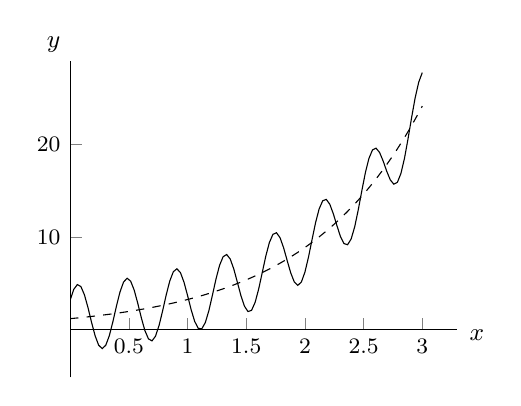
\begin{tikzpicture}
\begin{axis}[small,axis lines*=middle,xmin=0,ymax=29,xlabel={$x$},ylabel={$y$},xlabel style={at={(axis description cs:1.05,0.18)}},ylabel style={rotate={-90}},ylabel style={at={(axis description cs:0,1.05)}}]
\addplot[domain=0:3,samples=100]{1.2*e^(x)+2*cos(180/pi*15*x)+3*sin(180/pi*15*x)};
\addplot[dashed,domain=0:3,samples=100]{1.2*e^(x)};
\end{axis}
\end{tikzpicture}
\caption{مثال \حوالہ{مثال_سادہ_بلند_منفرد_مخلوط_جذر} کا مخصوص حل۔}
\label{شکل_مثال_سادہ_بلند_منفرد_مخلوط_جذر}
\end{figure}
\انتہا{مثال}
%==============================

\جزوحصہء{متعدد حقیقی جذر}
امتیازی مساوات کا دوہرا منفرد جذر \عددی{\lambda_1=\lambda_2} ہونے کی صورت میں، صفحہ \حوالہصفحہ{جدول_سادہ_دو_درجی_تین_صورتیں} پر  جدول \حوالہ{جدول_سادہ_دو_درجی_تین_صورتیں} کے تحت، تفرقی مساوات کے خطی طور غیر تابع حل \عددی{y=y_1} اور  \عددی{y_2=xy_1} ہوں گے۔ 

اسی حقیقت کے تحت اگر امتیازی مساوات کا  \عددی{m} گنا جذر \عددی{\lambda} پایا جائے تب تفرقی مساوات  کے \عددی{m} عدد خطی طور غیر تابع حل 
\begin{align}\label{مساوات_سادہ_بلند_متعدد_گنا_جذر_الف}
e^{\lambda x}, \, xe^{\lambda x}, \, x^2e^{\lambda x}, \cdots, x^{m-1}e^{\lambda x}
\end{align}
ہوں گے۔ایک مثال دیکھنے کے بعد درج بالا حل کو ثابت کرتے ہیں۔
%===================
\ابتدا{مثال}\quad حقیقی دہرا اور سہ گنا جذر\\
درج ذیل تفرقی مساوات کو حل کریں۔
\begin{align*}
y^{(5)}-8y^{(4)}+25y'''-38y''+28y'-8y=0
\end{align*}
حل:امتیازی مساوات \عددی{\lambda^5-8\lambda^4+25\lambda^3-38\lambda^2+28\lambda-8=0} کے جذر \عددی{\lambda_1=\lambda_2=1} اور \عددی{\lambda_3=\lambda_4=\lambda_5=2} ہیں۔یوں تفرقی مساوات کا عمومی حل
\begin{align*}
y=(c_1+c_2 x)e^x+(c_3+c_4x+c_5x^2)e^{2x}
\end{align*}
ہو گا۔
\انتہا{مثال}
%=====================

آئیں اب مساوات \حوالہ{مساوات_سادہ_بلند_متعدد_گنا_جذر_الف} کو ثابت کریں۔مساوات \حوالہ{مساوات_سادہ_بلند_مستقل_سر_متجانس_الف} کے بائیں ہاتھ کو
\begin{align*}
L[y]=y^{(n)}+a_{n-1}y^{(n-1)}+\cdots+a_0y
\end{align*}
لکھ کر اس میں \عددی{y=e^{\lambda x}} پر کرتے ہوئے تفرق لیتے ہیں۔
\begin{align*}
L[e^{\lambda x}]=(\lambda^n+a_{n-1}\lambda^{n-1}+\cdots+a_0)e^{\lambda x}
\end{align*}
اب تصور کریں کہ امتیازی مساوات کا \عددی{m} گنا جذر \عددی{\lambda_1} پایا جاتا ہے (جہاں \عددی{m<n} ہے) جبکہ بقایا، \عددی{\lambda_1} سے مختلف، جذر \عددی{\lambda_{m+1}} تا \عددی{\lambda_n} ہیں۔یوں کثیر رکنی کو اجزائے ضربی کی صورت میں لکھا جا سکتا ہے
\begin{align}\label{مساوات_سادہ_بلند_متعدد_گنا_جذر_ب}
L[e^{\lambda x}]=(\lambda-\lambda_1)^m(\lambda-\lambda_{m+1})(\lambda-\lambda_{m+2}) \cdots (\lambda-\lambda_n)e^{\lambda x}=(\lambda-\lambda_1)^m h(\lambda)e^{\lambda x}
\end{align}
جہاں \عددی{m=n} کی صورت  میں \عددی{h(\lambda)=1} ہو گا۔دونوں ہاتھ \عددی{\lambda} تفرق لیتے ہیں۔
\begin{align}\label{مساوات_سادہ_بلند_متعدد_گنا_جذر_پ}
\frac{\partial }{\partial \lambda} L[e^{\lambda x}]=m(\lambda-\lambda_1)^{m-1}h(\lambda)e^{\lambda x}+(\lambda-\lambda_1)^m \frac{\partial}{\partial \lambda}[h(\lambda)e^{\lambda x}]
\end{align}
اب چونکہ \عددی{x} تفرق اور \عددی{\lambda} تفرق غیر تابع  اور حاصل تفرق استمراری ہیں لہٰذا بائیں ہاتھ ان کی ترتیب بدلی جا سکتی ہے۔
\begin{align}\label{مساوات_سادہ_بلند_متعدد_گنا_جذر_ت}
\frac{\partial}{\partial \lambda} L[{e^{\lambda x}}]=L\left[\frac{\partial}{\partial \lambda} e^{\lambda x}\right]=L[xe^{\lambda x}]
\end{align}
چونکہ \عددی{\lambda_1} جذر \عددی{m} گنا ہے، جہاں \عددی{m\ge 2} ہے، لہٰذا  \عددی{\lambda=\lambda_1} پر مساوات \حوالہ{مساوات_سادہ_بلند_متعدد_گنا_جذر_پ} کے دائیں ہاتھ  کی قیمت جزو \عددی{(\lambda-\lambda_1)} کی بنا صفر ہو گی۔اس طرح  مساوات \حوالہ{مساوات_سادہ_بلند_متعدد_گنا_جذر_پ} اور مساوات \حوالہ{مساوات_سادہ_بلند_متعدد_گنا_جذر_ت} کو ملا کر \عددی{L[xe^{\lambda x}]=0} حاصل ہوتا ہے لہٰذا ثابت ہوا کہ \عددی{xe^{\lambda x}} مساوات \حوالہ{مساوات_سادہ_بلند_مستقل_سر_متجانس_الف} کا حل ہے۔

اسی ترتیب کو دہراتے ہوئے مساوات \حوالہ{مساوات_سادہ_بلند_متعدد_گنا_جذر_ب} کا دو درجی تفرق لیتے ہوئے \عددی{L[x^2e^{\lambda x}]=0} لکھا جا سکتا ہے جس سے ثابت ہوتا ہے کہ \عددی{x^2e^{\lambda x}} بھی مساوات \حوالہ{مساوات_سادہ_بلند_مستقل_سر_متجانس_الف} کا حل ہے۔اس ترکیب کو بار بار دہراتے ہوئے آخر کار \عددی{m-1} درجی تفرق لیتے ہیں۔
\begin{multline}\label{مساوات_سادہ_بلند_متعدد_گنا_جذر_ٹ}
\frac{\partial^{\, m-1} }{\partial \lambda^{m-1}} L[e^{\lambda x}]=L[x^{m-1}e^{\lambda x}]=m(m-1)(m-2)\cdots (3)(2)(\lambda-\lambda_1)^{1}h(\lambda)e^{\lambda x}\\
+(\lambda-\lambda_1)^m \frac{\partial^{\, m-1}}{\partial \lambda^{m-1}}[h(\lambda)e^{\lambda x}]
\end{multline}
مساوات کا دایاں ہاتھ \عددی{\lambda-\lambda_1} کی بنا \عددی{\lambda=\lambda_1} پر صفر کے برابر ہے لہٰذا اس سے \عددی{L[x^{m-1}e^{\lambda x}]=0} حاصل ہوتا ہے جس سے ثابت ہوتا ہے کہ \عددی{x^{m-1}e^{\lambda x}} بھی مساوات \حوالہ{مساوات_سادہ_بلند_مستقل_سر_متجانس_الف} کا حل ہے۔

مساوات \حوالہ{مساوات_سادہ_بلند_متعدد_گنا_جذر_ب} کا \عددی{m} درجی تفرق لینے کے لئے مساوات \حوالہ{مساوات_سادہ_بلند_متعدد_گنا_جذر_ٹ} کا تفرق لے سکتے ہیں جس سے
\begin{multline*}
\frac{\partial^m }{\partial \lambda^m} L[e^{\lambda x}]=L[x^me^{\lambda x}]=m(m-1)(m-2)\cdots (3)(2)(1)h(\lambda)e^{\lambda x}\\
+(\lambda-\lambda_1)^m \frac{\partial^m}{\partial \lambda^m}[h(\lambda)e^{\lambda x}]
\end{multline*}
ملتا ہے۔ مساوات کے دائیں ہاتھ پہلے جزو میں \عددی{\lambda-\lambda_1} کا جزو نہیں پایا جاتا لہٰذا \عددی{\lambda=\lambda_1} پر اس کی قیمت صفر کے برابر نہیں ہو گی۔یوں \عددی{L[x^me^{\lambda x}] \ne 0} ہو گا لہٰذا \عددی{x^me^{\lambda x}} تفرقی مساوات \حوالہ{مساوات_سادہ_بلند_مستقل_سر_متجانس_الف} کا حل نہیں ہو گا۔یوں مساوات \حوالہ{مساوات_سادہ_بلند_متعدد_گنا_جذر_الف} ثابت ہوتی ہے۔

آئیں اب ثابت کریں کہ مساوات \حوالہ{مساوات_سادہ_بلند_متعدد_گنا_جذر_الف} میں دیے گئے حل خطی طور غیر تابع ہیں۔مخصوص \عددی{m} کے لئے ان حل کا ورونسکی غیر صفر حاصل ہوتا ہے جس سے حل کی خطی طور غیر تابع ہونا ثابت ہوتا ہے۔کسی بھی \عددی{m} کی صورت میں ورونسکی کی \عددی{m} عدد  قالب سے \عددی{e^{\lambda x}} باہر نکالتے ہوئے  کل \عددی{e^{m\lambda x}} باہر نکالا جائے گا۔بقایا قالب میں مختلف صف آپس میں جمع اور منفی کرتے ہوئے قالب کی حتمی قیمت  \عددی{1}، \عددی{x}، \نقطے \عددی{x^{m-1}} کی ورونسکی کے برابر ثابت کی جا سکتی ہے جو غیر صفر مقدار ہے۔یہ تفاعل تفرقی مساوات \عددی{y^{(m)}=0} کے حل ہیں لہٰذا مسئلہ \حوالہ{مسئلہ_سادہ_بلند_حل_تابع_غیر_تابع} کے تحت یہ حل خطی طور غیر تابع ثابت ہوتے ہیں۔
%=========================

\جزوحصہء{متعدد مخلوط جذر}
مخلوط جذر کی جوڑیاں پائی جاتی ہیں۔یوں دوہرے مخلوط جذر کی صورت میں  \عددی{\lambda=\gamma+i\omega} اور \عددی{\bar{\lambda}=\gamma-i\omega} دو مرتبہ پائے جائیں گے جن سے 
\begin{align*}
e^{\gamma x+i\omega x}, \quad xe^{\gamma x+i\omega x}, \quad e^{\gamma x-i\omega x}, \quad xe^{\gamma x-i\omega x}
\end{align*}
حل لکھے جا سکتے ہیں۔ان سے حقیقی حل لکھتے ہیں۔
\begin{align}
e^{\gamma x}\cos \omega x,\quad  e^{\gamma x}\sin \omega x,\quad   xe^{\gamma x}\cos \omega x,\quad xe^{\gamma x}\sin \omega x 
\end{align}
بائیں جانب کے دو عدد حل \عددی{e^{\gamma x+i\omega x}} اور \عددی{e^{\gamma x-i\omega x}} جبکہ بقایا دو
 حل \عددی{xe^{\gamma x+i\omega x}} اور \عددی{xe^{\gamma x-i\omega x}}  سے حاصل کیے گئے ہیں۔ان سے عمومی حل لکھتے ہیں۔
\begin{align}
y=e^{\gamma x}[(A_1+A_2 x)\cos \omega x+(B_1+B_2 x)\sin \omega x]
\end{align}
مخلوط سہ گنا جذر (جو حقیقی مسائل میں شاذ و نادر  پایا جاتا ہے) کی صورت میں درج ذیل حقیقی حل حاصل ہوں گے۔
\begin{align*}
e^{\gamma x}\cos \omega x,\,\,  e^{\gamma x}\sin \omega x,\,\,   xe^{\gamma x}\cos \omega x,\,\, xe^{\gamma x}\sin \omega x,\,\,   x^2e^{\gamma x}\cos \omega x,\,\, x^2e^{\gamma x}\sin \omega x 
\end{align*}
اسی طرح آپ زیادہ تعداد میں پائے جانے والے مخلوط جذر سے بھی حل لکھ سکتے ہیں۔
%=======================

\حصہء{سوالات}


%===============
سوال \حوالہ{سوال_سادہ_بلند_عمومی_حل_الف} تا سوال \حوالہ{سوال_سادہ_بلند_عمومی_حل_ب} کے  عمومی حل لکھیں۔

%=================
\ابتدا{سوال}\شناخت{سوال_سادہ_بلند_عمومی_حل_الف}\quad
$y'''+4y'=0$\\
جواب:\عددی{y=c_1+c_2\cos 2x+c_3\sin 2x}
\انتہا{سوال}
%================
\ابتدا{سوال}\quad
$y^{(4)}+8y''+16y=0$\\
جواب:\عددی{y=c_1\cos 2x+c_2\sin 2x+c_3x\cos 2x+c_4x\sin 2x}
\انتہا{سوال}
%=================
\ابتدا{سوال}\quad
$y^{(4)}-y=0$\\
جواب:\عددی{y=c_1e^{x}+c_2e^{-x}+c_3\cos x+c_4\sin x}
\انتہا{سوال}
%==================
\ابتدا{سوال}\quad
$y^{(4)}+9y''=0$\\
جواب:\عددی{y=c_1+c_2x+c_3\cos 3x+c_4\sin 3x}
\انتہا{سوال}
%===================
\ابتدا{سوال}\quad
$y^{(5)}+y'''=0$\\
جواب:\عددی{y=c_1+c_2x+c_3x^2+c_4\cos x+c_5\sin x}
\انتہا{سوال}
%==================
\ابتدا{سوال}\quad 
$y^{(5)}-y^{(4)}-6y'''+14y''-11y'+3y=0$\\
جواب:\عددی{y=c_0e^{-3x}+c_1e^x+c_2xe^x+c3x^2e^x+c_4x^3e^{x}}
\انتہا{سوال}
%============================
\ابتدا{سوال}\شناخت{سوال_سادہ_بلند_عمومی_حل_ب}\quad
$y^{(5)}-2y^{(4)}-y'+2y=0$\\
جواب:\عددی{y=c_1e^{x}+c_2e^{-x}+c_3e^{2x}+c_4\cos x+c_5\sin x}
\انتہا{سوال}
%=================

سوال \حوالہ{سوال_سادہ_بلند_ابتدائی_قیمت_الف} تا سوال \حوالہ{سوال_سادہ_بلند_ابتدائی_قیمت_ب} ابتدائی قیمت مسئلوں کے حل دریافت کریں۔جذر حاصل کرنے کی خاطر کمپیوٹر استعمال کیا جا سکتا ہے۔

%========================
\ابتدا{سوال}\شناخت{سوال_سادہ_بلند_ابتدائی_قیمت_الف}\quad
$y'''-2.7y''-4.6y'+9.6y=0,\quad y(0)=1.5, \,y'(0)=2, \, y''(0)=-3$\\
جواب:\عددی{y=2.521e^{1.5x}-0.286e^{-2x}-0.735e^{3.2x}}
\انتہا{سوال}
%===============================
\ابتدا{سوال}
\begin{align*}
y'''+10.06y''-94.82y'-670.8766y&=0,\\
 y(0)=-1.2,\, y'(0)=5.2, \, y''(0)&=-2.8
\end{align*}
جواب:\عددی{y=0.229e^{-13.4x}-1.447e^{-5.6x}+0.018e^{8.94x}}
\انتہا{سوال}
%=========================
\ابتدا{سوال}\quad
$y'''+5y''+49y'+245y=0,\quad y(0)=10, \,y'(0)=-5, \, y''(0)=1$\\
جواب:\عددی{y=6.635e^{-5x}+3.365\cos 7x+4.025\sin 7x}
\انتہا{سوال}
%===============================
\ابتدا{سوال}\quad
$y'''+8y''+21y'+18y=0,\quad y(0)=2, \,y'(0)=1, \, y''(0)=-0.5$\\
جواب:\عددی{y=23.5e^{-2x}-21.5e^{-3x}-16.5xe^{-3x}}
\انتہا{سوال}
%===============================
\ابتدا{سوال}
\begin{align*}
y^{(4)}+8y''+16y&=0 \\
y(0)=1, \,y'(0)=0.5, \, y''(0)=-0.5,\, y'''(0)&=-1
\end{align*}
جواب:\عددی{y=\cos 2x+0.3125\sin 2x-0.125x\cos 2x+0.875x\sin 2x}
\انتہا{سوال}
%===============================
\ابتدا{سوال}\شناخت{سوال_سادہ_بلند_ابتدائی_قیمت_ب}
\begin{align*}
y^{(5)}-4y^{(4)}+8y'''-8y''+4y'&=0 \\
y(0)=1, \,y'(0)=0.5, \, y''(0)=-0.5,\, y'''(0)=-1, \, y^{(4)}&=2
\end{align*}
جواب:\عددی{y=0.5+0.5e^{x}\cos x+0.75e^x\sin x-0.75xe^x\cos x-0.25xe^x\sin x}
\انتہا{سوال}
%===============================
\ابتدا{سوال}\quad تخفیف درجہ\\
آپ تخفیف درجہ کے ذریعہ مثال \حوالہ{مثال_سادہ_دو_تخفیف_درجہ} میں دو درجی مساوات سے  کم درجی تفرقی مساوات حاصل کر چکے ہیں۔ مستقل عددی سر والے خطی متجانس سادہ تفرقی مساوات کا ایک حل \عددی{\lambda_1} جانتے ہوئے کم درجی مساوات کیسے حاصل کی جا سکتی ہے؟

جوابات:امتیازی مساوات کو \عددی{\lambda-\lambda_1}  سے تقسیم کرتے ہوئے کم درجی تفرقی مساوات کی امتیازی مساوات حاصل کی جا سکتی ہے جس سے کم درجی مساوات لکھی جا سکتی ہے۔
\انتہا{سوال}
%=====================
\ابتدا{سوال}\quad تخفیف درجہ\\
متغیر عددی سر والے خطی متجانس مساوات
\begin{align*}
y'''+p_2(x)y''+p_1(x)y'+p_0(x)y=0
\end{align*}
کا ایک حل \عددی{y_1} جانتے ہوئے دوسرے حل کو \عددی{y_2(x)=u(x)y_1(x)} لکھ کر، جہاں \عددی{u(x)=\int z(x)\dif x} ہے، درج بالا میں پر کرتے ہوئے کم درجی مساوات 
\begin{align*}
y_1z''+(3y_1'+p_2y_1)z'+(3y_1''+2p_2y_1'+p_1y_1)z=0
\end{align*}
حاصل کریں  ہے۔
\انتہا{سوال}
%=====================
\ابتدا{سوال}\quad تخفیف درجہ\\
تفرقی مساوات 
\begin{align*}
x^3y'''-3x^2y''+(6x-x^3)y'-(6-x^2)y=0
\end{align*}
کا ایک حل \عددی{y_1=x} ہے۔تخفیف درجہ سے دو درجی مساوات حاصل کریں۔

جواب:\عددی{z''-z=0}
\انتہا{سوال}
%===========================
%==========================

\حصہ{غیر متجانس خطی سادہ تفرقی مساوات}
آئیں اب معیاری صورت میں لکھی گئی، \عددی{n} درجی غیر متجانس خطی سادہ تفرقی مساوات
\begin{align}\label{مساوات_سادہ_بلند_غیر_متجانس_الف}
y^{(n)}+p_{n-1}(x)y^{(n-1)}+\cdots+p_1(x)y'+p_0(x)y=r(x)
\end{align}
پر غور کریں جہاں \عددی{y^{(n)}=\tfrac{\dif^{\, n} y}{\dif x^n}} اور \عددی{r(x) \not \equiv 0} ہیں۔کھلے وقفہ \عددی{I} پر مساوات \حوالہ{مساوات_سادہ_بلند_غیر_متجانس_الف} کا عمومی حل
\begin{align}\label{مساوات_سادہ_بلند_غیر_متجانس_ب}
y(x)=y_h(x)+y_p(x)
\end{align}
ہو گا جہاں \عددی{y_h(x)=c_1y_1(x)+c_2y_2(x)+\cdots c_ny_n(x)} مطابقتی متجانس خطی تفرقی مساوات
\begin{align}\label{مساوات_سادہ_بلند_مطابقتی_متجانس_الف}
y^{(n)}+p_{n-1}(x)y^{(n-1)}+\cdots+p_1(x)y'+p_0(x)y=0
\end{align}
کا \عددی{I} پر عمومی حل ہے۔ \عددی{y_p(x)} مساوات \حوالہ{مساوات_سادہ_بلند_غیر_متجانس_الف}  کا \عددی{I} پر  ایسا کوئی بھی حل ہے جس میں اختیاری مستقل نہ پایا جاتا ہو۔ کھلے وقفہ \عددی{I} پر مساوات \حوالہ{مساوات_سادہ_بلند_غیر_متجانس_الف} کے استمراری عددی سر اور استمراری \عددی{r(x)} کی صورت میں \عددی{I} پر مساوات \حوالہ{مساوات_سادہ_بلند_غیر_متجانس_الف} کا عمومی حل موجود ہے جس میں مساوات \حوالہ{مساوات_سادہ_بلند_غیر_متجانس_الف} کے تمام حل موجود ہیں۔یوں مساوات \حوالہ{مساوات_سادہ_بلند_غیر_متجانس_الف} کا کوئی نادر حل نہیں پایا جاتا ہے۔

مساوات \حوالہ{مساوات_سادہ_بلند_غیر_متجانس_الف} پر مبنی ابتدائی قیمت مسئلہ مساوات \حوالہ{مساوات_سادہ_بلند_غیر_متجانس_الف} اور درج ذیل \عددی{n-1} ابتدائی شرائط پر مبنی ہو گا جہاں \عددی{x_0} کھلے وقفے \عددی{x_0} پر پایا جاتا ہے۔تفرقی مساوات کے عددی سر اور \عددی{r} کھلے وقفے پر استمراری ہونے کی صورت میں اس ابتدائی قیمت مسئلے کا حل \اصطلاح{یکتا} ہو گا۔ حل کے یکتائی کو حصہ \حوالہ{حصہ_سادہ_دو_غیر_متجانس} میں دو درجی تفرقی مساوات کے یکتا حل کے ثبوت کے نمونے پر ثابت کیا جا سکتا ہے۔
\begin{align}
y(x_0)=K_0, \quad y'(x_0)=K_1, \cdots , y^{(n-1)}(x_0)=K_{n-1}
\end{align}
%=====================
\جزوحصہء{نا معلوم عددی سر کی ترکیب}
غیر متجانس تفرقی مساوات \حوالہ{مساوات_سادہ_بلند_غیر_متجانس_الف} کے عمومی حل کے لئے مساوات \حوالہ{مساوات_سادہ_بلند_غیر_متجانس_الف} کا مخصوص حل درکار ہو گا۔مستقل عددی سر والی تفرقی مساوات،
\begin{align}\label{مساوات_سادہ_بلند_مستقل_عددی_سر_غیر_متجانس_الف}
y^{(n)}+a_{n-1}y^{(n-1)}+\cdots+a_1y'+a_0 y=r(x)
\end{align}
جہاں \عددی{a_0} تا \عددی{a_{n-1}} مستقل مقدار اور \عددی{r(x)}، حصہ \حوالہ{حصہ_سادہ_دو_غیر_متجانس} کی طرح، خاص نوعیت کا تفاعل ہو، کا مخصوص حل  حصہ \حوالہ{حصہ_سادہ_دو_غیر_متجانس} کی طرح، بذریعہ \اصطلاح{نا معلوم عددی سر کی ترکیب}\فرہنگ{نا معلوم عددی سر کی ترکیب} حاصل کیا جا سکتا ہے۔مخصوص حل \عددی{y_p} کو جبری تفاعل \عددی{r} سے درج ذیل قواعد کے تحت لکھا جاتا ہے۔
%=====================================================
\begin{enumerate}
\item[بنیادی قاعدہ:]\label{قاعدہ_سادہ_بلند_بنیادی_قاعدہ}
یہ قاعدہ حصہ \حوالہ{حصہ_سادہ_دو_غیر_متجانس} میں دیے قاعدے  کی طرح ہے۔
\item[ترمیمی قاعدہ:]\label{قاعدہ_سادہ_بلند_ترمیمی_قاعدہ}
اگر \عددی{r} کو دیکھ کر چنے گئے \عددی{y_p}  کا کوئی رکن   مساوات \حوالہ{مساوات_سادہ_بلند_مستقل_عددی_سر_غیر_متجانس_الف} کے  مطابقتی متجانس مساوات کا حل \عددی{y_k} ہو تب  اس رکن کی جگہ \عددی{x^ky_k} کو  \عددی{y_p} میں شامل کریں، جہاں \عددی{k} ایسا کم سے کم قیمت کا مثبت عدد ہے کہ تفاعل \عددی{x^ky_k} مطابقتی متجانس مساوات کا حل نہ ہو۔
\item[مجموعے کا قاعدہ:]\label{قاعدہ_سادہ_بلند_مجموعہ_قاعدہ}
یہ قاعدہ حصہ \حوالہ{حصہ_سادہ_دو_غیر_متجانس} میں دیے قاعدے کی طرح ہے۔
\end{enumerate} 
 %=============================================

موجودہ ترکیب میں \عددی{k=1} یا \عددی{k=2} سے حصہ \حوالہ{حصہ_سادہ_دو_غیر_متجانس} کی ترکیب حاصل ہوتی ہے۔آئیں مثال کی مدد سے موجودہ ترکیب کا ترمیمی قاعدہ  استعمال کرنا سیکھیں۔

%=================
\ابتدا{مثال}\quad ابتدائی قیمت مسئلہ۔ ترمیمی قاعدہ۔
درج ذیل ابتدائی قیمت مسئلہ حل کریں۔
\begin{align*}
y'''-3y''+3y'-y=e^{x}, \quad y(0)=8, \quad y'(0)=-2, \quad y''(0)=-5
\end{align*}

حل:پہلا قدم: \quad مطابقتی متجانس مساوات کا امتیازی مساوات \عددی{\lambda^3-3\lambda^2+3\lambda-1=0} ہے جس کو \عددی{(\lambda-1)^3=0} لکھا جا سکتا ہے جس سے سہ گنا جذر \عددی{\lambda=1} ملتا ہے۔یوں  متجانس مساوات کو عمومی حل
\begin{align*}
y_h=c_1e^x+c_2xe^x+c_3x^2e^x
\end{align*}
لکھا جا سکتا ہے۔

دوسرا قدم:\quad اب اگر ہم دیے گئے غیر متجانس مساوات کے جبری تفاعل کو دیکھ کر \عددی{y_p=Ce^x} چنتے ہوئے \عددی{y_p} اور اس کے تفرقات کو دیے گئے مساوات میں پر  کریں تو \عددی{C-3C+3C-C=1} ملتا ہے جس سے \عددی{C} کی قیمت حاصل نہیں کی جا سکتی ہے۔اس کا مطلب ہے کہ چننا گیا \عددی{y_p} دیے گئے تفرقی مساوات پر پورا نہیں اترتا لہٰذا اس  \عددی{y_p} کو رد کرنا ہو گا۔آپ \عددی{y_p=Cxe^x} یا \عددی{y_p=Cx^2e^x} چن کر دیکھ سکتے ہیں کہ یہ تفاعل بھی دیے گئے تفرقی مساوات پر پورا نہیں اترتے۔یوں ہم اوپر دیے گئے ترمیمی قاعدے کے تحت \عددی{y_p=Cx^3e^x} چنتے ہیں جس کے تفرقات درج ذیل ہیں۔
\begin{align*}
y'&=Ce^x(x^3+3x^2)\\
y''&=Ce^x(x^3+6x^2+6x)\\
y'''&=Ce^x(x^3+9x^2+18x+6)
\end{align*}
\عددی{y_p} اور اس کے تفرقات کو دیے گئے تفرقی مساوات میں پر کرتے 

\begin{align*}
Ce^x(x^3+9x^2+18x+6)-3Ce^x(x^3+6x^2+6x)+3Ce^x(x^3+3x^2)-Cx^3e^x=e^{x}
\end{align*}
ہوئے \عددی{C=\tfrac{1}{6}} ملتا ہے۔یوں دیے گئے غیر متجانس تفرقی مساوات کا مخصوص حل \عددی{y_p=\tfrac{1}{6}x^3e^x} ہے لہٰذا اس کا عمومی حل درج ذیل ہو گا۔
\begin{align*}
y=y_h+y_p=c_1e^x+c_2xe^x+c_3x^2e^x+\frac{1}{6}x^3e^x
\end{align*}
تیسرا قدم:\quad مخصوص حل حاصل کرنے کی خاطر عمومی حل کے مستقل حاصل کرنے ہوں گے۔عمومی حل میں پہلی ابتدائی معلومات \عددی{y(0)=8} پر کرتے ہوئے \عددی{c_1=8} ملتا ہے۔اس قیمت کو \عددی{y} میں پر کرتے ہوئے \عددی{y'} لے کر دوسری ابتدائی معلومات \عددی{y'(0)=-2} سے \عددی{c_2} حاصل ہوتی ہے۔اسی طرح \عددی{y'''} لیتے ہوئے اس میں \عددی{y'''(0)=-5} پر کرتے ہوئے \عددی{c_3} کی قیمت حاصل ہوتی ہے۔
\begin{align*}
y&=(c_1+c_2x+c_3x^2+\frac{1}{6}x^3)e^x, \quad y(0)=8, \quad y(0)=8=c_1\\
y'&=(c_1+c_2+c_2x+c_3x^2+2c_3x+\frac{x^3}{6}+\frac{x^2}{2})e^x, \quad y'(0)=-2, \quad c_2=-10\\
y''&=(c_1+2c_2+2c_3+c_2x+4c_3x+c_3x^2+\frac{x^3}{6}+\frac{5}{6}x^2+x)e^x,\,y''(0)=-5, \, c_3=\frac{7}{2}
\end{align*} 
ان قیمتوں کو استعمال کرتے ہوئے مخصوص حل لکھتے ہیں۔
\begin{align*}
y=\left(8-10x+\frac{7}{2}x^2+\frac{x^3}{6}\right)e^x
\end{align*}
\انتہا{مثال}
%========================
\حصہ{متعین متغیرات بدلنے کے طریقے سے  غیر متجانس خطی سادہ تفرقی مساوات کا حل}\شناخت{سادہ_بلند_متغیرات_بدلنے_کا_طریقہ}
متعین متغیرات بدلنے کا طریقہ (حصہ \حوالہ{سادہ_دو_متغیرات_بدلنے_کا_طریقہ} دیکھیں) بلند درجی تفرقی مساوات  کے لئے بھی قابل استعمال ہے۔یوں معیاری صورت میں لکھے گئے خطی غیر متجانس سادہ تفرقی مساوات  \حوالہ{مساوات_سادہ_بلند_غیر_متجانس_الف}، جس کے عددی سر اور \عددی{r(x)} کھلے وقفہ \عددی{I} پر استمراری ہوں، کا  \عددی{I} پر مخصوص حل \عددی{y_p} درج ذیل ہو گا۔
\begin{gather}
\begin{aligned}\label{مساوات_سادہ_بلند_متعین_متغیرات_بدلنے_الف}
y_p(x)&=\sum_{k=1}^{n} y_k(x)\int \frac{W_k(x)}{W(x)} r(x)\dif x\\
&=y_1(x)\int \frac{W_1(x)}{W(x)}r(x)\dif x+\cdots+y_n(x)\int \frac{W_n(x)}{W(x)}r(x)\dif x
\end{aligned}
\end{gather}
مساوات \حوالہ{مساوات_سادہ_بلند_متعین_متغیرات_بدلنے_الف} میں \عددی{y_1} تا \عددی{y_n} مطابقتی متجانس مساوات \حوالہ{مساوات_سادہ_بلند_مطابقتی_متجانس_الف} کے حل کی اساس ہیں جبکہ ورونسکی \عددی{W} کے \عددی{k} قطار میں \عددی{[0\,\,0\,\cdots\,0\,\,1]^T} پر کرتے ہوئے \عددی{W_k} حاصل کی جاتی ہے۔یوں \عددی{n=2} کی صورت میں \عددی{W}، \عددی{W_1} اور \عددی{W_2} درج ذیل ہوں گے۔
\begin{align*}
W=
\begin{vmatrix}
y_1& y_2\\[1mm]
y_1'&y_2'
\end{vmatrix}, \quad
W_1=
\begin{vmatrix}
0&y_2\\[1mm]
1&y_2'
\end{vmatrix}=-y_2, \quad
W_2=
\begin{vmatrix}
y_1& 0\\[1mm]
y_1'&1
\end{vmatrix}=y_1
\end{align*}

مساوات \حوالہ{مساوات_سادہ_بلند_متعین_متغیرات_بدلنے_الف} کو صفحہ \حوالہصفحہ{مساوات_سادہ_دو_غیر_متجانس_خطی_ب} پر دیے  گئے 
 مساوات \حوالہ{مساوات_سادہ_دو_غیر_متجانس_خطی_ب} کی ثبوت کی طرز پر ثابت کیا جا سکتا ہے۔
%========================
\ابتدا{مثال}\شناخت{مثال_سادہ_بلند_یولر_کوشی_بدل}متعین متغیرات کی تبدیلی۔یولر کوشی غیر متجانس مساوات\\
درج ذیل غیر متجانس یولر کوشی مساوات کو حل کریں۔
\begin{align*}
x^3y'''-3x^2y''+6xy'-6y=x^4\ln x , \quad (x>0) 
\end{align*}

حل: پہلا قدم:\quad مطابقتی متجانس مساوات میں \عددی{y=x^m} اور اس کے تفرقات  پر کرتے ہوئے
\begin{align*}
[m(m-1)(m-1)-3m(m-1)+6m-6]x^m=0
\end{align*}
ملتا ہے جس کو \عددی{x^m} سے تقسیم کرتے ہوئے  جذر \عددی{1}، \عددی{2} اور \عددی{3} حاصل ہوتے ہیں۔ان جذر سے اساس
\begin{align*}
y_1=x, \quad y_2=x^2,\quad y_3=x^3
\end{align*}
لکھتے ہیں۔یوں متجانس یولر کوشی مساوات کا عمومی حل درج ذیل ہو گا۔
\begin{align*}
y=c_1x+c_2x^2+c_3x^3
\end{align*}
دوسرا قدم:\quad مساوات \حوالہ{مساوات_سادہ_بلند_متعین_متغیرات_بدلنے_الف} میں درکار قالب کی حتمی قیمتیں حاصل کرتے ہیں۔
\begin{align*}
W=
\begin{vmatrix}
x & x^2 & x^3\\
1 & 2x & 3x^2\\
0 & 2 &  6x
\end{vmatrix}=2x^3, \quad
W_1=
\begin{vmatrix}
0 & x^2 & x^3\\
0 & 2x & 3x^2\\
1 & 2 &  6x
\end{vmatrix}=x^4\\
W_2=
\begin{vmatrix}
x & 0 & x^3\\
1 & 0 & 3x^2\\
0 & 1 &  6x
\end{vmatrix}=-2x^3, \quad
W_3=
\begin{vmatrix}
x & x^2 &0\\
1 & 2x & 0\\
0 & 2 &  1
\end{vmatrix}=x^2
\end{align*}
تیسرا قدم:\quad مساوات \حوالہ{مساوات_سادہ_بلند_متعین_متغیرات_بدلنے_الف} کے تکمل میں \عددی{r(x)} بھی درکار ہے جو دیے گئے یولر کوشی مساوات کو معیاری صورت میں لکھنے سے ملتا ہے۔دیے گئے مساوات کو \عددی{y'''} کے عددی سر  \عددی{x^3} سے تقسیم کرتے ہوئے تفرقی مساوات کی معیاری صورت حاصل ہوتی ہے جس سے \عددی{r=x\ln x} ملتا ہے۔مساوات \حوالہ{مساوات_سادہ_بلند_متعین_متغیرات_بدلنے_الف}  میں \عددی{\tfrac{W_1}{W}=\tfrac{x}{2}}، \عددی{\tfrac{W_2}{W}=-1} اور
 \عددی{\tfrac{W_3}{W}=\tfrac{1}{2x}} ہیں لہٰذا 
\begin{align*}
y_p&=x\int \frac{x}{2} x\ln x \dif x-x^2\int x\ln x \dif x+x^3\int \frac{1}{2x} x\ln x \dif x\\
&=\frac{x}{2}\left(\frac{x^3}{3}\ln x -\frac{x^3}{9}\right)-x^2\left(\frac{x^2}{2}\ln x-\frac{x^2}{4}\right)+\frac{x^3}{2}\left(x\ln x-x\right)\\
&=\frac{1}{6}x^4\left(\ln x-\frac{11}{6}\right)
\end{align*}
ہو گا۔یوں عمومی حل درج ذیل ہو گا۔\عددی{y_p} کو شکل \حوالہ{شکل_مثال_سادہ_بلند_یولر_کوشی_بدل} میں دکھایا گیا ہے۔
\begin{align*}
y=y_h+y_p=c_1x+c_2x^2+c_3x^3+\frac{1}{6}x^4\left(\ln x-\frac{11}{6}\right)
\end{align*}
%
\begin{figure}
\centering
\begin{tikzpicture}
\begin{axis}[small, axis lines*=middle,xmin=0,xlabel={$x$},ylabel={$y_p$},ylabel style={rotate=-90},ylabel style={at={(axis description cs:0,1.05)}},xlabel style={at={(axis description cs:1.05,0.5)}}]
\addplot[domain=0:6.7,samples=50]{1/6*x^4*(ln(x)-11/6)};
\end{axis}
\end{tikzpicture}
\caption{مثال \حوالہ{مثال_سادہ_بلند_یولر_کوشی_بدل} کا \عددی{y_p}}
\label{شکل_مثال_سادہ_بلند_یولر_کوشی_بدل}
\end{figure}
\انتہا{مثال}
%========================

\جزوحصہء{عملی استعمال۔لچکدار شہتیر}
دو درجی تفرقی مساوات کا عملی انجینئری میں بہت زیادہ استعمال پایا جاتا ہے البتہ بلند درجی تفرقی مساوات عملی انجینئری کے بہت کم مسائل میں کام آتے ہیں۔ انجینئری کا ایک انتہائی اہم مسئلہ لچکدار شہتیر کا جھکا و ہے جس کی نمونہ کشی  چہارم درجی تفرقی مساوات کرتی ہے۔کسی بھی عمارت یا پل میں شہتیر کلیدی کردار ادا کرتے ہیں جو لکڑی یا لوہے کے ہو سکتے ہیں۔
%====================
\ابتدا{مثال}\شناخت{مثال_سادہ_بلند_شہتیر_کا_جھکاو}
شکل \حوالہ{شکل_مثال_سادہ_بلند_شہتیر_کا_جھکاو}-الف میں، یکساں لچک کے مادے سے بنا ہوا، مستطیل رقبہ عمودی تراش کا شہتیر دکھایا گیا ہے جس کی لمبائی \عددی{L} ہے۔شہتیر کی اپنی وزن سے شہتیر کے جھکاو کو رد کیا جا سکتا ہے۔شکل-ب میں شہتیر کے \عددی{x} محور پر عمودی بیرونی بوجھ \عددی{f(x)} ڈالا گیا ہے جس کی وجہ سے شہتیر میں جھکاو پیدا ہوا ہے۔بیرونی بوجھ اور شہتیر کی جھکاو کا تعلق، علم لچک کے تحت، درج ذیل ہے  جہاں \عددی{E} \اصطلاح{ینگ کا مقیاس لچک}\فرہنگ{ینگ!مقیاس اثر}\فرہنگ{مقیاس اثر!ینگ}\حاشیہب{Young's modulus of elasticity}\فرہنگ{Young's modulus of elasticity}\فرہنگ{modulus of elasticity!Young's} کہلاتا ہے جبکہ \عددی{I} مستطیل کا \عددی{z} محور پر \اصطلاح{جمودی معیار اثر}\فرہنگ{جمودی معیار اثر}\فرہنگ{معیار اثر!جمودی}\حاشیہب{moment of inertia}\فرہنگ{moment of inertia} ہے۔شہتیر کی فی اکائی لمبائی پر بیرونی قوت کو بوجھ \عددی{f(x)} لکھا گیا ہے۔ 
\begin{align}\label{مساوات_سادہ_بلند_شہتیر_کا_جھکاو_الف}
EIy^{(4)}=f(x)
\end{align}


\begin{figure}
\centering
\begin{subfigure}{0.5\textwidth}
\centering
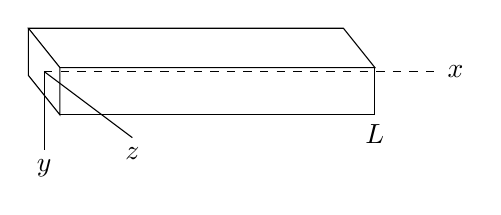
\begin{tikzpicture}
\pgfmathsetmacro{\kx}{4}
\pgfmathsetmacro{\kdx}{0.4}
\pgfmathsetmacro{\ky}{0.5}
\pgfmathsetmacro{\kdy}{0.6}
\pgfmathsetmacro{\kang}{acos(\kdx/\ky)}
%beam
\draw(0,0)--++(\kx,0)--++(-\kdx,\ky)--++(-\kx,0)--++(\kdx,-\ky);
\draw(-\kdx,\ky)--++(0,-\kdy)--++(\kdx,-\ky)--++(0,\kdy);
\draw(0,-\kdy)--++(\kx,0)node[below]{$L$}--++(0,\kdy);
%axis
\draw(-\kdx/2,\ky/2-\kdy/2)--++(0,-1)node[below]{$y$};
\draw[dashed](-\kdx/2,\ky/2-\kdy/2)--++(\kx+1,0)node[right]{$x$};
\draw(-\kdx/2,\ky/2-\kdy/2)--++(-\kang:1.4)node[below]{$z$};
\end{tikzpicture}
\caption*{(الف) مستطیل رقبہ عمودی تراش کا شہتیر جس کی لمبائی \عددی{L} ہے۔}
\end{subfigure}%
\begin{subfigure}{0.5\textwidth}
\centering
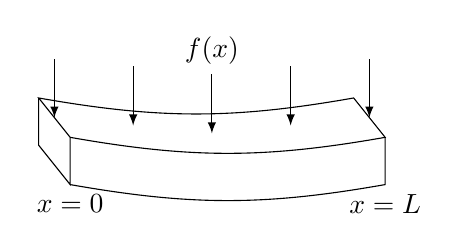
\begin{tikzpicture}
\pgfmathsetmacro{\kx}{4}
\pgfmathsetmacro{\kdx}{0.4}
\pgfmathsetmacro{\ky}{0.5}
\pgfmathsetmacro{\kdy}{0.6}
\pgfmathsetmacro{\kang}{acos(\kdx/\ky)}
%beam
\draw(0,0)to [out=-10,in=-170]++(\kx,0)--++(-\kdx,\ky) to [out=-170,in=-10]++(-\kx,0)--++(\kdx,-\ky);
\draw(-\kdx,\ky)--++(0,-\kdy)--++(\kdx,-\ky)--++(0,\kdy);
\draw(0,-\kdy)node[below]{$x=0$} to [out=-10,in=-170]++(\kx,0)node[below]{$x=L$}--++(0,\kdy);
%load
\draw[latex-](-\kdx/2,\ky/2)--++(0,0.75);
\draw[latex-](\kx-\kdx/2,\ky/2)--++(0,0.75);
\draw[latex-](\kx/4-\kdx/2,\ky/2-0.1)--++(0,0.75);
\draw[latex-](3/4*\kx-\kdx/2,\ky/2-0.1)--++(0,0.75);
\draw[latex-](\kx/2-\kdx/2,\ky/2-0.2)--++(0,0.75)node[above]{$f(x)$};
\end{tikzpicture}
\caption*{(ب) بوجھ شہتیر کو چھکا دیتی ہے۔}
\end{subfigure}%
\caption{مثال \حوالہ{مثال_سادہ_بلند_شہتیر_کا_جھکاو} کا شہتیر۔}
\label{شکل_مثال_سادہ_بلند_شہتیر_کا_جھکاو}
\end{figure}%
%%%%%%%%%%%%%%
\begin{figure}
\centering
\begin{subfigure}{0.5\textwidth}
\centering
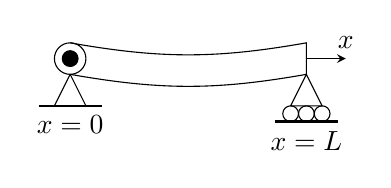
\begin{tikzpicture}
\pgfmathsetmacro{\kx}{3}
\pgfmathsetmacro{\ky}{0.4}
%beam
\draw(0,0) to [out=-10,in=-170]++(\kx,0)--++(0,\ky) to [out=-170,in=-10]++(-\kx,0);
\draw(0,\ky/2) circle (\ky/2);
\draw[fill](0,\ky/2) circle (1mm);
\draw[-stealth] (\kx,\ky/2)--++(0.5,0)node[above]{$x$};
%wedges
\draw(0,0)--++(0.2,-0.4)--++(-0.4,0)--++(0.2,0.4);
\draw(\kx,0)--++(0.2,-0.4)--++(-0.4,0)--++(0.2,0.4);
%foundations
\draw[thick](-0.4,-0.4)--++(0.4+0.4,0);
\draw[thick](\kx-0.4,-0.4-0.2)--++(0.4+0.4,0);
\draw(0,-0.4)node[below]{$x=0$};
\draw(\kx,-0.4-0.2)node[below]{$x=L$};
%wheels
\draw(\kx-0.2,-0.4-0.1) circle (0.1);
\draw(\kx,-0.4-0.1) circle (0.1);
\draw(\kx+0.2,-0.4-0.1) circle (0.1);
\end{tikzpicture}
\caption*{(الف) سادہ سہارا دیا گیا ہے۔}
\end{subfigure}
\begin{subfigure}{0.5\textwidth}
\centering
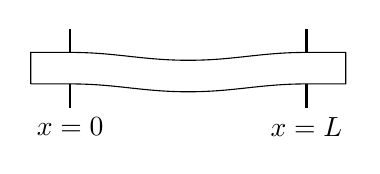
\begin{tikzpicture}
\pgfmathsetmacro{\kx}{3}
\pgfmathsetmacro{\ky}{0.4}
\pgfmathsetmacro{\kdx}{0.5}
%beam clamped at both ends
\draw(-\kdx,0)--++(\kdx,0) to [out=0,in=180]++(\kx/2,-\ky/4) to [out=0,in=180]++(\kx/2,\ky/4)--++(\kdx,0)--++(0,\ky)--++(-\kdx,0) to [out=180,in=0]++(-\kx/2,-\ky/4) to [out=180,in=0]++(-\kx/2,\ky/4)--++(-\kdx,0)--++(0,-\ky);
%end clamps
\draw[thick](0,0)--++(0,-0.3)node[below]{$x=0$};
\draw[thick](0,\ky)--++(0,0.3);
\draw[thick](\kx,0)--++(0,-0.3)node[below]{$x=L$};
\draw[thick](\kx,\ky)--++(0,0.3);
\end{tikzpicture}
\caption*{(ب) دونوں اطراف سے جکڑا ہوا۔}
\end{subfigure}
\begin{subfigure}{0.5\textwidth}
\centering
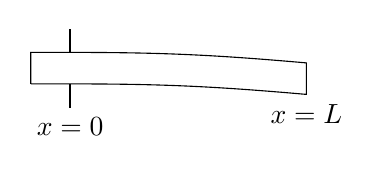
\begin{tikzpicture}
\pgfmathsetmacro{\kx}{3}
\pgfmathsetmacro{\ky}{0.4}
\pgfmathsetmacro{\kdx}{0.5}
%beam clamped at both ends
\draw(-\kdx,0)--++(\kdx,0) to [out=0,in=175]++(\kx,-\ky/3)node[below]{$x=L$}--++(0,\ky) to [out=175,in=0]++(-\kx,\ky/3)--++(-\kdx,0)--++(0,-\ky);
%end clamps
\draw[thick](0,0)--++(0,-0.3)node[below]{$x=0$};
\draw[thick](0,\ky)--++(0,0.3);
\end{tikzpicture}
\caption*{(پ) ایک طرف سے جکڑا گیا ہے۔}
\end{subfigure}%
\caption{شہتیر جکڑنے کے عمومی طریقے۔}
\label{شکل_شہتیر_جکڑا_گیا_ہے}
\end{figure}%

شہتیر کو عموماً شکل \حوالہ{شکل_شہتیر_جکڑا_گیا_ہے} میں دکھائے گئے تین طریقوں سے  نصب کیا جاتا ہے جو درج ذیل سرحدی شرائط کو جنم دیتے ہیں۔
\begin{itemize}
\item[(الف)]\quad سادہ سہارا \quad
$y(0)=y(L)=y''(0)=y''(L)=0$
\item[(ب)]\quad دونوں اطراف جکڑے گئے ہیں \quad 
$y(0)=y(L)=y'(0)=y'(L)=0$
\item[(پ)]\quad ایک طرف جکڑا گیا ہے \quad
$y(0)=y'(0)=y''(L)=y'''(L)=0$
\end{itemize}
سرحدی  شرط \عددی{y=0} سے مراد صفر ہٹاو ہے، \عددی{y'=0} سے مراد افقی مماس ہے، \عددی{y''=0} سے مراد صفر  \اصطلاح{خماو کا معیار اثر}\فرہنگ{معیار اثر!خماو}\فرہنگ{خماو!معیار اثر}\حاشیہب{bending moment}\فرہنگ{bending moment}\فرہنگ{moment!bending} ہے جبکہ \عددی{y'''=0} سے مراد صفر \اصطلاح{جزی قوت}\فرہنگ{جزی قوت}\فرہنگ{قوت!جزی}\حاشیہب{shearing force}\فرہنگ{shearing force} ہے۔

آئیں سادہ سہارے والی شہتیر کے مسئلے کو حل کریں جسے شکل \حوالہ{شکل_شہتیر_جکڑا_گیا_ہے}-الف میں دکھایا گیا ہے۔یکساں بیرونی بوجھ کی صورت میں \عددی{f(x)=f_0} ہو گا اور مساوات \حوالہ{مساوات_سادہ_بلند_شہتیر_کا_جھکاو_الف} درج ذیل صورت اختیار کرے گی
\begin{align}
y^{(4)}=k, \quad k=\frac{f_0}{EI}
\end{align}
جس کو تکمل کے ذریعہ حل کرتے ہیں۔دو مرتبہ تکمل لیتے ہیں۔
\begin{align*}
y''=\frac{k}{2}x^2+c_1x+c_2
\end{align*}
\عددی{y''(0)=0} پر کرتے ہوئے \عددی{c_2=0} حاصل ہوتا ہے جس کے بعد  \عددی{y''(L)=0} پر کرنے سے \عددی{c_1-\tfrac{kL}{2}} ملتا ہے۔یوں
\begin{align*}
y''=\frac{k}{2}x^2-\frac{kL}{2}x
\end{align*}
ہو گا جس کا دو مرتبہ تکمل لینے سے درج ذیل حاصل ہوتا ہے۔
\begin{align*}
y=\frac{k}{2}\left(\frac{1}{12}x^4-\frac{L}{6}x^3+c_3x+c_4\right)
\end{align*}
\عددی{y(0)=0} پر کرنے سے \عددی{c_4=0} ملتا ہے جس کے بعد \عددی{y(L)=0} پر کرتے ہوئے \عددی{c_3} حاصل کرتے ہیں۔
\begin{align*}
y(L)=\frac{kL}{2}\left(\frac{L^3}{12}-\frac{L^3}{6}+c_3\right)=0, \quad c_3=\frac{L^3}{12}
\end{align*}
یوں \عددی{k=\tfrac{f_0}{EI}} لکھتے ہوئے شہتیر کی لچک بالمقابل لمبائی درج ذیل ہو گی۔
\begin{align*}
y(x)=\frac{f_0}{24EI}(x^4-2Lx^3+L^3x)
\end{align*}
ہم توقع رکھتے ہیں کہ شہتیر کے درمیان سے دونوں اطراف یکساں جھکاو پایا جائے گا یعنی \عددی{y(x)=y(L-x)} ہو گا۔زیادہ سے زیادہ جھکاو \عددی{y(\tfrac{L}{2})=\tfrac{5f_0L^4}{16\times 24EI}} ہے جو \عددی{x=\tfrac{L}{2}} پر پایا جاتا ہے۔یاد رہے کہ شکل \حوالہ{شکل_مثال_سادہ_بلند_شہتیر_کا_جھکاو} میں مثبت \عددی{y} نیچے کی طرف کو ہے۔
\انتہا{مثال}
%=====================

\حصہء{سوالات}
سوال \حوالہ{سوال_سادہ_بلند_غیر_متجانس_الف} تا سوال \حوالہ{سوال_سادہ_بلند_غیر_متجانس_ب} کو حل کریں۔

%==================
\ابتدا{سوال}\شناخت{سوال_سادہ_بلند_غیر_متجانس_الف}\quad
$y^{(4)}+3y'''-4y=0$\\
جواب:\عددی{y=c_1e^x+c_2e^{-x}+c_3\cos 2x+c_4\sin 2x}
\انتہا{سوال}
%=======================
\ابتدا{سوال}\quad
$y'''+16y''+13y'=0$\\
جواب:\عددی{y=c_1+c_2e^{-3x}\cos 2x+c_3e^{-3x}\sin 2x}
\انتہا{سوال}
%=======================
\ابتدا{سوال}\quad
$y'''+3y''-y'-3y=5e^{2x}$\\
جواب:\عددی{y=c_1e^x+c_2e^{-x}+c_3e^{-3x}+\tfrac{1}{3}e^{2x}}
\انتہا{سوال}
%=======================
\ابتدا{سوال}\quad
$y^{(4)}+8y''-9y=\cosh 2x$\\
جواب:\عددی{y=c_1e^x+c_2e^{-x}+c_3\cos 3x+c_4\sin 3x+\tfrac{5}{39}\cosh 2x}
\انتہا{سوال}
%=======================
\ابتدا{سوال}\quad
$x^2y'''+3xy''-2y'=0$\\
جواب:\عددی{y=c_1+c_2x^{\sqrt{3}}+c_3x^{-\sqrt{3}}}
\انتہا{سوال}
%=======================
\ابتدا{سوال}\quad
$y'''+2.25y''+1.6875y'+0.421875y=0$\\
جواب:\عددی{y=c_1e^{-0.75x}+c_2xe^{-0.75x}+c_3x^2e^{-0.75x}}
\انتہا{سوال}
%=======================
\ابتدا{سوال}\quad
$y'''-y'=\frac{3}{40}\sinh \frac{x}{2}$\\
جواب:\عددی{y=c_1+c_2e^x+c_3e^{-x}-2\cosh \tfrac{x}{2}}
\انتہا{سوال}
%=======================
\ابتدا{سوال}\شناخت{سوال_سادہ_بلند_غیر_متجانس_ب}\quad
$y'''+9y''+27y'+27=2x^2$\\
جواب:\عددی{y=c_1e^{-3x}+c_2xe^{-3x}+c_3x^2e^{-3x}+\tfrac{2}{27}x^2-\tfrac{4}{27}x+\tfrac{8}{81}}
\انتہا{سوال}
%=======================
سوال \حوالہ{سوال_سادہ_بلند_ابتدائی_الف} تا سوال \حوالہ{سوال_سادہ_بلند_ابتدائی_ب} ابتدائی قیمت مسئلے ہیں۔ انہیں حل کریں۔

%==================
\ابتدا{سوال}\شناخت{سوال_سادہ_بلند_ابتدائی_الف} 
\begin{align*}
y^{(4)}-10y''+9y=4e^{-2x}\\
y(0)=1, \quad y'(0)=-1,\quad y''(0)=-0.5,\quad y'''(0)=0.2
\end{align*}
جواب:\عددی{y=-\tfrac{2}{15}e^{-2x}+\tfrac{1}{1440}(127e^x+1383e^{-x}-119e^{3x}-271e^{-3x})}
\انتہا{سوال}
%========================
\ابتدا{سوال}
\begin{align*}
y^{(4)}+y''-2y=0.5\sin 2x\\
y(0)=2, \quad y'(0)=-1,\quad y''(0)=-1,\quad y'''(0)=2
\end{align*}
جواب:\عددی{y=0.05\sin 2x+3\cos x-0.358\sin x-\cos \sqrt{2}x-0.424\sin \sqrt{2}x}
\انتہا{سوال}
%========================
\ابتدا{سوال}
مطابقتی متجانس مساوات  کا حل \عددی{y_h} حاصل کرتے ہوئے \عددی{W}، \عددی{W_1}، \عددی{W_2}  اور \عددی{W_3} قالبوں کی حتمی قیمتیں حاصل کریں۔انہیں استعمال کرتے ہوئے غیر متجانس مساوات حل کریں۔(یاد رہے تفرقی مساوات کو معیاری صورت میں لکھتے ہوئے \عددی{r=x} حاصل ہو گا) 
\begin{align*}
x^3y'''-5x^2y''+12xy'-12y=x^4, \,\quad y(1)=1,\, y'(1)=-1,\,y''(1)=2
\end{align*}
جوابات:\عددی{y_h=c_1x+c_2x^3+c_3x^4}، \عددی{W=6x^5}، \عددی{W_1=x^6}، \عددی{W_2=-3x^4}، \عددی{W_3=2x^3}\\
\عددی{y=\tfrac{59}{18}x-\tfrac{9}{2}x^3+\tfrac{8}{3}x^4+\tfrac{x^4}{3}\ln x-\tfrac{4}{9}x^4}
\انتہا{سوال}
%=============================
\ابتدا{سوال}
مطابقتی متجانس مساوات  کا حل \عددی{y_h} حاصل کرتے ہوئے \عددی{W}، \عددی{W_1}، \عددی{W_2}  اور \عددی{W_3} قالبوں کی حتمی قیمتیں حاصل کریں۔انہیں استعمال کرتے ہوئے غیر متجانس مساوات حل کریں۔
\begin{align*}
x^3y'''+5x^2y''+2xy'-2y=x^2, \,\quad y(1)=2,\, y'(1)=1,\,y''(1)=-1
\end{align*}
جوابات:\عددی{y_h=c_1x^{-1}+c_2x+c_3x^{-2}}، \عددی{W=6x^{-5}}، \عددی{W_1=-3x^{-2}}، \عددی{W_2=x^{-4}}، \عددی{W_3=2x^{-1}}، 
\عددی{y=\tfrac{5}{3x}+x-\tfrac{3}{4x^2}+\tfrac{x^2}{12}}
\انتہا{سوال}
%=============================
\ابتدا{سوال}\شناخت{سوال_سادہ_بلند_ابتدائی_ب}
\begin{align*}
y'''+9y''+27y'+27y=27x^2, \quad y(0)=2,\, y'(0)=-1,\, y''(0)=-1
\end{align*}
جواب:\عددی{y=\tfrac{2}{3}e^{-3x}+3xe^{-3x}+\tfrac{9}{2}x^2e^{-3x}+x^2-2x+\tfrac{4}{3}}
\انتہا{سوال}
%========================
